% CVPR 2026 author kit (github.com/cvpr-org/author-kit, tag CVPR2026-v1)
\documentclass[10pt,twocolumn,letterpaper]{article}
\usepackage{cvpr}              % camera-ready layout: names shown, no line numbers
\usepackage[T1]{fontenc}
\usepackage[utf8]{inputenc}
\usepackage{microtype}

\setlength{\textfloatsep}{8pt plus 2pt minus 2pt}
\setlength{\dbltextfloatsep}{8pt plus 2pt minus 2pt}

% generated by pathfaith.make_numbers -- do not edit by hand
\newcommand{\wnMrr}{0.484}
\newcommand{\wnHitsOne}{0.415}
\newcommand{\wnHitsThree}{0.520}
\newcommand{\wnHitsTen}{0.617}
\newcommand{\wnBaseN}{3134}
\newcommand{\wnNodes}{40{,}943}
\newcommand{\wnEdges}{173{,}670}
\newcommand{\wnQueries}{200}
\newcommand{\wnScanned}{288}
\newcommand{\wnPool}{20}
\newcommand{\wnRelCount}{11}
\newcommand{\wnTopk}{5}
\newcommand{\wnComprehensiveness}{0.1722}
\newcommand{\wnComprehensivenessCI}{[0.1460, 0.1988]}
\newcommand{\wnComprehensivenessRandom}{0.0000}
\newcommand{\wnComprehensivenessRandomCI}{[0.0000, 0.0000]}
\newcommand{\wnCompMinusRandom}{0.1721}
\newcommand{\wnCompMinusRandomCI}{[0.1460, 0.1988]}
\newcommand{\wnSufficiency}{0.0251}
\newcommand{\wnSufficiencyCI}{[0.0201, 0.0305]}
\newcommand{\wnBaseProb}{0.1750}
\newcommand{\wnBaseProbCI}{[0.1489, 0.2014]}
\newcommand{\wnSingleEdgeDrop}{0.1240}
\newcommand{\wnSingleEdgeDropCI}{[0.1018, 0.1472]}
\newcommand{\wnRewireDropOnGold}{0.1622}
\newcommand{\wnRewireDropOnGoldCI}{[0.1358, 0.1892]}
\newcommand{\wnRewireGainOnTarget}{0.0282}
\newcommand{\wnRewireGainOnTargetCI}{[0.0209, 0.0357]}
\newcommand{\wnTopOneIsBest}{0.253}
\newcommand{\wnTopOneIsBestCI}{[0.196, 0.314]}
\newcommand{\wnTopOneChance}{0.280}
\newcommand{\wnTopOneChanceCI}{[0.234, 0.327]}
\newcommand{\wnTopOneOverChance}{\ensuremath{-}0.028}
\newcommand{\wnTopOneOverChanceCI}{[\ensuremath{-}0.080, 0.026]}
\newcommand{\wnCompFracOfBase}{0.858}
\newcommand{\wnCompFracOfBaseCI}{[0.813, 0.898]}
\newcommand{\wnCompRandomFracOfBase}{0.000}
\newcommand{\wnCompRandomFracOfBaseCI}{[0.000, 0.000]}
\newcommand{\wnBottleneckFrac}{0.884}
\newcommand{\wnBottleneckFracCI}{[0.856, 0.909]}
\newcommand{\wnDistinctEdgeRatio}{0.248}
\newcommand{\wnDistinctEdgeRatioCI}{[0.226, 0.271]}
\newcommand{\wnSingleEdgeRecoversFrac}{0.650}
\newcommand{\wnSingleEdgeRecoversFracCI}{[0.581, 0.716]}
\newcommand{\wnSuffFracOfBase}{0.313}
\newcommand{\wnSuffFracOfBaseCI}{[0.248, 0.390]}
\newcommand{\wnKendallTauGradVsDrop}{\ensuremath{-}0.009}
\newcommand{\wnKendallTauGradVsDropCI}{[\ensuremath{-}0.054, 0.037]}
\newcommand{\wnTopMinusBottom}{\ensuremath{-}0.003}
\newcommand{\wnTopMinusBottomCI}{[\ensuremath{-}0.013, 0.007]}
\newcommand{\wnMeanDropTopQuartile}{0.147}
\newcommand{\wnMeanDropTopQuartileCI}{[0.125, 0.169]}
\newcommand{\wnMeanDropBottomQuartile}{0.150}
\newcommand{\wnMeanDropBottomQuartileCI}{[0.127, 0.174]}
\newcommand{\wnFracRankBroken}{76.0}
\newcommand{\wnFracRankBrokenCI}{[70.0, 81.5]}
\newcommand{\wnFracSingleEdgeBreaks}{45.0}
\newcommand{\wnFracSingleEdgeBreaksCI}{[38.0, 52.0]}
\newcommand{\wnFracRewireFollowed}{75.5}
\newcommand{\wnFracRewireFollowedCI}{[69.5, 81.0]}
\newcommand{\wnFracCompNegative}{1.5}
\newcommand{\wnFracCompNegativeCI}{[0.0, 3.5]}
\newcommand{\wnFracCompMeaningful}{93.0}
\newcommand{\wnFracCompMeaningfulCI}{[89.5, 96.5]}
\newcommand{\wnFracSuffAboveOne}{8.0}
\newcommand{\wnFracSuffAboveOneCI}{[4.5, 12.0]}
\newcommand{\wnFracPoolTied}{8.5}
\newcommand{\wnRewireAsymmetry}{5.7}
\newcommand{\wnRankAfter}{252}
\newcommand{\wnForwards}{26.2}
\newcommand{\wnPaths}{18.3}
\newcommand{\wnDistinctEdges}{34.5}
\newcommand{\wnSeconds}{17.8}
\newcommand{\wnRevN}{115}
\newcommand{\wnRevCompFracOfBase}{0.984}
\newcommand{\wnRevCompFracOfBaseCI}{[0.967, 0.998]}
\newcommand{\wnRevSuffFracOfBase}{0.148}
\newcommand{\wnRevSuffFracOfBaseCI}{[0.124, 0.175]}
\newcommand{\wnRevBottleneckFrac}{0.894}
\newcommand{\wnRevBottleneckFracCI}{[0.868, 0.918]}
\newcommand{\wnRevDistinctEdgeRatio}{0.186}
\newcommand{\wnRevDistinctEdgeRatioCI}{[0.175, 0.198]}
\newcommand{\wnRevSingleEdgeRecoversFrac}{0.807}
\newcommand{\wnRevSingleEdgeRecoversFracCI}{[0.729, 0.875]}
\newcommand{\wnRevKendallTauGradVsDrop}{\ensuremath{-}0.012}
\newcommand{\wnRevKendallTauGradVsDropCI}{[\ensuremath{-}0.069, 0.045]}
\newcommand{\wnRevRewireDropOnGold}{0.2808}
\newcommand{\wnRevRewireDropOnGoldCI}{[0.2494, 0.3132]}
\newcommand{\wnRevRewireGainOnTarget}{0.0474}
\newcommand{\wnRevRewireGainOnTargetCI}{[0.0363, 0.0593]}
\newcommand{\wnRevTopOneIsBest}{0.157}
\newcommand{\wnRevTopOneIsBestCI}{[0.096, 0.226]}
\newcommand{\wnRevTopOneChance}{0.217}
\newcommand{\wnRevTopOneChanceCI}{[0.168, 0.269]}
\newcommand{\wnRevFracSingleEdgeBreaks}{56.5}
\newcommand{\wnRevFracSingleEdgeBreaksCI}{[47.0, 65.2]}
\newcommand{\wnNoRevN}{85}
\newcommand{\wnNoRevCompFracOfBase}{0.688}
\newcommand{\wnNoRevCompFracOfBaseCI}{[0.600, 0.771]}
\newcommand{\wnNoRevSuffFracOfBase}{0.536}
\newcommand{\wnNoRevSuffFracOfBaseCI}{[0.398, 0.697]}
\newcommand{\wnNoRevBottleneckFrac}{0.872}
\newcommand{\wnNoRevBottleneckFracCI}{[0.817, 0.920]}
\newcommand{\wnNoRevDistinctEdgeRatio}{0.333}
\newcommand{\wnNoRevDistinctEdgeRatioCI}{[0.289, 0.379]}
\newcommand{\wnNoRevSingleEdgeRecoversFrac}{0.395}
\newcommand{\wnNoRevSingleEdgeRecoversFracCI}{[0.286, 0.506]}
\newcommand{\wnNoRevKendallTauGradVsDrop}{\ensuremath{-}0.003}
\newcommand{\wnNoRevKendallTauGradVsDropCI}{[\ensuremath{-}0.082, 0.077]}
\newcommand{\wnNoRevRewireDropOnGold}{0.0017}
\newcommand{\wnNoRevRewireDropOnGoldCI}{[0.0010, 0.0027]}
\newcommand{\wnNoRevRewireGainOnTarget}{0.0023}
\newcommand{\wnNoRevRewireGainOnTargetCI}{[0.0002, 0.0059]}
\newcommand{\wnNoRevTopOneIsBest}{0.392}
\newcommand{\wnNoRevTopOneIsBestCI}{[0.291, 0.506]}
\newcommand{\wnNoRevTopOneChance}{0.372}
\newcommand{\wnNoRevTopOneChanceCI}{[0.288, 0.460]}
\newcommand{\wnNoRevFracSingleEdgeBreaks}{29.4}
\newcommand{\wnNoRevFracSingleEdgeBreaksCI}{[20.0, 40.0]}
\newcommand{\wnRevPct}{57.5}
\newcommand{\wnFwdPct}{0.0}
\newcommand{\wnTailDegMedian}{13}
\newcommand{\wnTailDegMin}{2}
\newcommand{\wnTailLeafPct}{6.5}
\newcommand{\wnSingleEdgeRecoversHiDeg}{0.613}
\newcommand{\wnSingleEdgeRecoversHiDegCI}{[0.538, 0.685]}
\newcommand{\wnHiDegN}{187}
\newcommand{\fbMrr}{0.371}
\newcommand{\fbHitsOne}{0.276}
\newcommand{\fbHitsThree}{0.406}
\newcommand{\fbHitsTen}{0.558}
\newcommand{\fbBaseN}{2000}
\newcommand{\fbNodes}{14{,}541}
\newcommand{\fbEdges}{544{,}230}
\newcommand{\fbQueries}{200}
\newcommand{\fbScanned}{400}
\newcommand{\fbPool}{20}
\newcommand{\fbRelCount}{237}
\newcommand{\fbTopk}{5}
\newcommand{\fbComprehensiveness}{0.0479}
\newcommand{\fbComprehensivenessCI}{[0.0335, 0.0643]}
\newcommand{\fbComprehensivenessRandom}{0.0000}
\newcommand{\fbComprehensivenessRandomCI}{[0.0000, 0.0001]}
\newcommand{\fbCompMinusRandom}{0.0479}
\newcommand{\fbCompMinusRandomCI}{[0.0335, 0.0642]}
\newcommand{\fbSufficiency}{0.1052}
\newcommand{\fbSufficiencyCI}{[0.0932, 0.1174]}
\newcommand{\fbBaseProb}{0.3633}
\newcommand{\fbBaseProbCI}{[0.3085, 0.4187]}
\newcommand{\fbSingleEdgeDrop}{0.0039}
\newcommand{\fbSingleEdgeDropCI}{[0.0000, 0.0100]}
\newcommand{\fbRewireDropOnGold}{0.0185}
\newcommand{\fbRewireDropOnGoldCI}{[0.0143, 0.0233]}
\newcommand{\fbRewireGainOnTarget}{0.0173}
\newcommand{\fbRewireGainOnTargetCI}{[0.0133, 0.0218]}
\newcommand{\fbTopOneIsBest}{0.080}
\newcommand{\fbTopOneIsBestCI}{[0.045, 0.120]}
\newcommand{\fbTopOneChance}{0.057}
\newcommand{\fbTopOneChanceCI}{[0.053, 0.062]}
\newcommand{\fbTopOneOverChance}{0.023}
\newcommand{\fbTopOneOverChanceCI}{[\ensuremath{-}0.012, 0.064]}
\newcommand{\fbCompFracOfBase}{0.259}
\newcommand{\fbCompFracOfBaseCI}{[0.212, 0.303]}
\newcommand{\fbCompRandomFracOfBase}{0.000}
\newcommand{\fbCompRandomFracOfBaseCI}{[0.000, 0.000]}
\newcommand{\fbBottleneckFrac}{0.734}
\newcommand{\fbBottleneckFracCI}{[0.701, 0.768]}
\newcommand{\fbDistinctEdgeRatio}{0.484}
\newcommand{\fbDistinctEdgeRatioCI}{[0.464, 0.503]}
\newcommand{\fbSingleEdgeRecoversFrac}{0.025}
\newcommand{\fbSingleEdgeRecoversFracCI}{[\ensuremath{-}0.014, 0.066]}
\newcommand{\fbSuffFracOfBase}{2.764}
\newcommand{\fbSuffFracOfBaseCI}{[1.681, 4.242]}
\newcommand{\fbKendallTauGradVsDrop}{0.048}
\newcommand{\fbKendallTauGradVsDropCI}{[0.010, 0.085]}
\newcommand{\fbTopMinusBottom}{\ensuremath{-}0.001}
\newcommand{\fbTopMinusBottomCI}{[\ensuremath{-}0.004, 0.002]}
\newcommand{\fbMeanDropTopQuartile}{0.022}
\newcommand{\fbMeanDropTopQuartileCI}{[0.015, 0.030]}
\newcommand{\fbMeanDropBottomQuartile}{0.022}
\newcommand{\fbMeanDropBottomQuartileCI}{[0.014, 0.032]}
\newcommand{\fbFracRankBroken}{17.0}
\newcommand{\fbFracRankBrokenCI}{[12.0, 22.5]}
\newcommand{\fbFracSingleEdgeBreaks}{1.0}
\newcommand{\fbFracSingleEdgeBreaksCI}{[0.0, 2.5]}
\newcommand{\fbFracRewireFollowed}{92.0}
\newcommand{\fbFracRewireFollowedCI}{[88.0, 95.5]}
\newcommand{\fbFracCompNegative}{4.5}
\newcommand{\fbFracCompNegativeCI}{[2.0, 7.5]}
\newcommand{\fbFracCompMeaningful}{68.0}
\newcommand{\fbFracCompMeaningfulCI}{[61.5, 74.0]}
\newcommand{\fbFracSuffAboveOne}{36.5}
\newcommand{\fbFracSuffAboveOneCI}{[30.0, 43.0]}
\newcommand{\fbFracPoolTied}{0.0}
\newcommand{\fbRewireAsymmetry}{1.1}
\newcommand{\fbRankAfter}{3}
\newcommand{\fbForwards}{27.9}
\newcommand{\fbPaths}{20.0}
\newcommand{\fbDistinctEdges}{59.1}
\newcommand{\fbSeconds}{47.0}
\newcommand{\fbNoRevN}{200}
\newcommand{\fbNoRevCompFracOfBase}{0.259}
\newcommand{\fbNoRevCompFracOfBaseCI}{[0.212, 0.303]}
\newcommand{\fbNoRevSuffFracOfBase}{2.764}
\newcommand{\fbNoRevSuffFracOfBaseCI}{[1.681, 4.242]}
\newcommand{\fbNoRevBottleneckFrac}{0.734}
\newcommand{\fbNoRevBottleneckFracCI}{[0.701, 0.768]}
\newcommand{\fbNoRevDistinctEdgeRatio}{0.484}
\newcommand{\fbNoRevDistinctEdgeRatioCI}{[0.464, 0.503]}
\newcommand{\fbNoRevSingleEdgeRecoversFrac}{0.025}
\newcommand{\fbNoRevSingleEdgeRecoversFracCI}{[\ensuremath{-}0.014, 0.066]}
\newcommand{\fbNoRevKendallTauGradVsDrop}{0.048}
\newcommand{\fbNoRevKendallTauGradVsDropCI}{[0.010, 0.085]}
\newcommand{\fbNoRevRewireDropOnGold}{0.0185}
\newcommand{\fbNoRevRewireDropOnGoldCI}{[0.0143, 0.0233]}
\newcommand{\fbNoRevRewireGainOnTarget}{0.0173}
\newcommand{\fbNoRevRewireGainOnTargetCI}{[0.0133, 0.0218]}
\newcommand{\fbNoRevTopOneIsBest}{0.080}
\newcommand{\fbNoRevTopOneIsBestCI}{[0.045, 0.120]}
\newcommand{\fbNoRevTopOneChance}{0.057}
\newcommand{\fbNoRevTopOneChanceCI}{[0.053, 0.062]}
\newcommand{\fbNoRevFracSingleEdgeBreaks}{1.0}
\newcommand{\fbNoRevFracSingleEdgeBreaksCI}{[0.0, 2.5]}
\newcommand{\fbRevPct}{0.0}
\newcommand{\fbFwdPct}{0.0}
\newcommand{\fbTailDegMedian}{854}
\newcommand{\fbTailDegMin}{14}
\newcommand{\fbTailLeafPct}{0.0}
\newcommand{\fbSingleEdgeRecoversHiDeg}{\ensuremath{-}0.015}
\newcommand{\fbSingleEdgeRecoversHiDegCI}{[\ensuremath{-}0.128, 0.056]}
\newcommand{\fbHiDegN}{200}
\newcommand{\cxMrr}{0.464}
\newcommand{\cxHitsOne}{0.361}
\newcommand{\cxHitsThree}{0.514}
\newcommand{\cxHitsTen}{0.665}
\newcommand{\cxBaseN}{1828}
\newcommand{\cxNodes}{2{,}034}
\newcommand{\cxEdges}{65{,}776}
\newcommand{\cxQueries}{200}
\newcommand{\cxScanned}{274}
\newcommand{\cxPool}{20}
\newcommand{\cxRelCount}{42}
\newcommand{\cxTopk}{5}
\newcommand{\cxComprehensiveness}{0.0590}
\newcommand{\cxComprehensivenessCI}{[0.0476, 0.0719]}
\newcommand{\cxComprehensivenessRandom}{0.0000}
\newcommand{\cxComprehensivenessRandomCI}{[\ensuremath{-}0.0001, 0.0002]}
\newcommand{\cxCompMinusRandom}{0.0590}
\newcommand{\cxCompMinusRandomCI}{[0.0476, 0.0718]}
\newcommand{\cxSufficiency}{0.3766}
\newcommand{\cxSufficiencyCI}{[0.3410, 0.4112]}
\newcommand{\cxBaseProb}{0.1880}
\newcommand{\cxBaseProbCI}{[0.1559, 0.2236]}
\newcommand{\cxSingleEdgeDrop}{0.0042}
\newcommand{\cxSingleEdgeDropCI}{[0.0021, 0.0066]}
\newcommand{\cxRewireDropOnGold}{0.0180}
\newcommand{\cxRewireDropOnGoldCI}{[0.0143, 0.0217]}
\newcommand{\cxRewireGainOnTarget}{0.0121}
\newcommand{\cxRewireGainOnTargetCI}{[0.0094, 0.0150]}
\newcommand{\cxTopOneIsBest}{0.125}
\newcommand{\cxTopOneIsBestCI}{[0.080, 0.175]}
\newcommand{\cxTopOneChance}{0.053}
\newcommand{\cxTopOneChanceCI}{[0.052, 0.055]}
\newcommand{\cxTopOneOverChance}{0.072}
\newcommand{\cxTopOneOverChanceCI}{[0.028, 0.120]}
\newcommand{\cxCompFracOfBase}{0.427}
\newcommand{\cxCompFracOfBaseCI}{[0.386, 0.470]}
\newcommand{\cxCompRandomFracOfBase}{0.000}
\newcommand{\cxCompRandomFracOfBaseCI}{[\ensuremath{-}0.001, 0.001]}
\newcommand{\cxBottleneckFrac}{0.721}
\newcommand{\cxBottleneckFracCI}{[0.686, 0.756]}
\newcommand{\cxDistinctEdgeRatio}{0.512}
\newcommand{\cxDistinctEdgeRatioCI}{[0.491, 0.533]}
\newcommand{\cxSingleEdgeRecoversFrac}{0.143}
\newcommand{\cxSingleEdgeRecoversFracCI}{[0.093, 0.197]}
\newcommand{\cxSuffFracOfBase}{4.754}
\newcommand{\cxSuffFracOfBaseCI}{[4.056, 5.505]}
\newcommand{\cxKendallTauGradVsDrop}{0.076}
\newcommand{\cxKendallTauGradVsDropCI}{[0.043, 0.108]}
\newcommand{\cxTopMinusBottom}{0.003}
\newcommand{\cxTopMinusBottomCI}{[0.001, 0.005]}
\newcommand{\cxMeanDropTopQuartile}{0.033}
\newcommand{\cxMeanDropTopQuartileCI}{[0.025, 0.043]}
\newcommand{\cxMeanDropBottomQuartile}{0.031}
\newcommand{\cxMeanDropBottomQuartileCI}{[0.023, 0.039]}
\newcommand{\cxFracRankBroken}{32.5}
\newcommand{\cxFracRankBrokenCI}{[26.0, 39.0]}
\newcommand{\cxFracSingleEdgeBreaks}{12.5}
\newcommand{\cxFracSingleEdgeBreaksCI}{[8.0, 17.5]}
\newcommand{\cxFracRewireFollowed}{94.0}
\newcommand{\cxFracRewireFollowedCI}{[90.5, 97.0]}
\newcommand{\cxFracCompNegative}{3.0}
\newcommand{\cxFracCompNegativeCI}{[1.0, 5.5]}
\newcommand{\cxFracCompMeaningful}{89.0}
\newcommand{\cxFracCompMeaningfulCI}{[84.5, 93.0]}
\newcommand{\cxFracSuffAboveOne}{81.0}
\newcommand{\cxFracSuffAboveOneCI}{[75.5, 86.5]}
\newcommand{\cxFracPoolTied}{0.0}
\newcommand{\cxRewireAsymmetry}{1.5}
\newcommand{\cxRankAfter}{4}
\newcommand{\cxForwards}{26.0}
\newcommand{\cxPaths}{20.0}
\newcommand{\cxDistinctEdges}{62.5}
\newcommand{\cxSeconds}{5.2}
\newcommand{\cxRevN}{26}
\newcommand{\cxRevCompFracOfBase}{0.805}
\newcommand{\cxRevCompFracOfBaseCI}{[0.746, 0.858]}
\newcommand{\cxRevSuffFracOfBase}{3.044}
\newcommand{\cxRevSuffFracOfBaseCI}{[2.140, 4.030]}
\newcommand{\cxRevBottleneckFrac}{0.985}
\newcommand{\cxRevBottleneckFracCI}{[0.965, 0.996]}
\newcommand{\cxRevDistinctEdgeRatio}{0.337}
\newcommand{\cxRevDistinctEdgeRatioCI}{[0.323, 0.350]}
\newcommand{\cxRevSingleEdgeRecoversFrac}{0.975}
\newcommand{\cxRevSingleEdgeRecoversFracCI}{[0.964, 0.985]}
\newcommand{\cxRevKendallTauGradVsDrop}{\ensuremath{-}0.012}
\newcommand{\cxRevKendallTauGradVsDropCI}{[\ensuremath{-}0.073, 0.051]}
\newcommand{\cxRevRewireDropOnGold}{0.0339}
\newcommand{\cxRevRewireDropOnGoldCI}{[0.0232, 0.0454]}
\newcommand{\cxRevRewireGainOnTarget}{0.0026}
\newcommand{\cxRevRewireGainOnTargetCI}{[0.0011, 0.0046]}
\newcommand{\cxRevTopOneIsBest}{0.000}
\newcommand{\cxRevTopOneIsBestCI}{[0.000, 0.000]}
\newcommand{\cxRevTopOneChance}{0.060}
\newcommand{\cxRevTopOneChanceCI}{[0.052, 0.067]}
\newcommand{\cxRevFracSingleEdgeBreaks}{96.2}
\newcommand{\cxRevFracSingleEdgeBreaksCI}{[88.5, 100.0]}
\newcommand{\cxNoRevN}{174}
\newcommand{\cxNoRevCompFracOfBase}{0.371}
\newcommand{\cxNoRevCompFracOfBaseCI}{[0.329, 0.413]}
\newcommand{\cxNoRevSuffFracOfBase}{5.010}
\newcommand{\cxNoRevSuffFracOfBaseCI}{[4.248, 5.858]}
\newcommand{\cxNoRevBottleneckFrac}{0.681}
\newcommand{\cxNoRevBottleneckFracCI}{[0.645, 0.717]}
\newcommand{\cxNoRevDistinctEdgeRatio}{0.538}
\newcommand{\cxNoRevDistinctEdgeRatioCI}{[0.517, 0.559]}
\newcommand{\cxNoRevSingleEdgeRecoversFrac}{0.001}
\newcommand{\cxNoRevSingleEdgeRecoversFracCI}{[\ensuremath{-}0.012, 0.018]}
\newcommand{\cxNoRevKendallTauGradVsDrop}{0.089}
\newcommand{\cxNoRevKendallTauGradVsDropCI}{[0.054, 0.124]}
\newcommand{\cxNoRevRewireDropOnGold}{0.0156}
\newcommand{\cxNoRevRewireDropOnGoldCI}{[0.0120, 0.0195]}
\newcommand{\cxNoRevRewireGainOnTarget}{0.0135}
\newcommand{\cxNoRevRewireGainOnTargetCI}{[0.0104, 0.0168]}
\newcommand{\cxNoRevTopOneIsBest}{0.144}
\newcommand{\cxNoRevTopOneIsBestCI}{[0.092, 0.195]}
\newcommand{\cxNoRevTopOneChance}{0.052}
\newcommand{\cxNoRevTopOneChanceCI}{[0.051, 0.053]}
\newcommand{\cxNoRevFracSingleEdgeBreaks}{0.0}
\newcommand{\cxNoRevFracSingleEdgeBreaksCI}{[0.0, 0.0]}
\newcommand{\cxRevPct}{13.0}
\newcommand{\cxFwdPct}{0.0}
\newcommand{\cxTailDegMedian}{320}
\newcommand{\cxTailDegMin}{24}
\newcommand{\cxTailLeafPct}{0.0}
\newcommand{\cxSingleEdgeRecoversHiDeg}{0.130}
\newcommand{\cxSingleEdgeRecoversHiDegCI}{[0.082, 0.181]}
\newcommand{\cxHiDegN}{200}
\newcommand{\nlMrr}{0.258}
\newcommand{\nlHitsOne}{0.172}
\newcommand{\nlHitsThree}{0.284}
\newcommand{\nlHitsTen}{0.431}
\newcommand{\nlBaseN}{4952}
\newcommand{\nlNodes}{22{,}925}
\newcommand{\nlEdges}{50{,}890}
\newcommand{\nlQueries}{200}
\newcommand{\nlScanned}{396}
\newcommand{\nlPool}{20}
\newcommand{\nlRelCount}{200}
\newcommand{\nlTopk}{5}
\newcommand{\nlComprehensiveness}{0.0612}
\newcommand{\nlComprehensivenessCI}{[0.0442, 0.0802]}
\newcommand{\nlComprehensivenessRandom}{0.0009}
\newcommand{\nlComprehensivenessRandomCI}{[0.0006, 0.0013]}
\newcommand{\nlCompMinusRandom}{0.0603}
\newcommand{\nlCompMinusRandomCI}{[0.0434, 0.0792]}
\newcommand{\nlSufficiency}{0.0294}
\newcommand{\nlSufficiencyCI}{[0.0195, 0.0400]}
\newcommand{\nlBaseProb}{0.1265}
\newcommand{\nlBaseProbCI}{[0.1007, 0.1543]}
\newcommand{\nlSingleEdgeDrop}{0.0078}
\newcommand{\nlSingleEdgeDropCI}{[0.0006, 0.0171]}
\newcommand{\nlRewireDropOnGold}{0.0466}
\newcommand{\nlRewireDropOnGoldCI}{[0.0270, 0.0676]}
\newcommand{\nlRewireGainOnTarget}{0.0430}
\newcommand{\nlRewireGainOnTargetCI}{[0.0260, 0.0630]}
\newcommand{\nlTopOneIsBest}{0.306}
\newcommand{\nlTopOneIsBestCI}{[0.245, 0.372]}
\newcommand{\nlTopOneChance}{0.307}
\newcommand{\nlTopOneChanceCI}{[0.259, 0.356]}
\newcommand{\nlTopOneOverChance}{0.000}
\newcommand{\nlTopOneOverChanceCI}{[\ensuremath{-}0.056, 0.056]}
\newcommand{\nlCompFracOfBase}{0.368}
\newcommand{\nlCompFracOfBaseCI}{[0.290, 0.444]}
\newcommand{\nlCompRandomFracOfBase}{0.007}
\newcommand{\nlCompRandomFracOfBaseCI}{[0.006, 0.010]}
\newcommand{\nlBottleneckFrac}{0.658}
\newcommand{\nlBottleneckFracCI}{[0.611, 0.704]}
\newcommand{\nlDistinctEdgeRatio}{0.295}
\newcommand{\nlDistinctEdgeRatioCI}{[0.274, 0.317]}
\newcommand{\nlSingleEdgeRecoversFrac}{0.086}
\newcommand{\nlSingleEdgeRecoversFracCI}{[0.026, 0.147]}
\newcommand{\nlSuffFracOfBase}{1.707}
\newcommand{\nlSuffFracOfBaseCI}{[0.936, 2.659]}
\newcommand{\nlKendallTauGradVsDrop}{0.041}
\newcommand{\nlKendallTauGradVsDropCI}{[\ensuremath{-}0.023, 0.102]}
\newcommand{\nlTopMinusBottom}{0.023}
\newcommand{\nlTopMinusBottomCI}{[0.012, 0.037]}
\newcommand{\nlMeanDropTopQuartile}{0.038}
\newcommand{\nlMeanDropTopQuartileCI}{[0.025, 0.054]}
\newcommand{\nlMeanDropBottomQuartile}{0.015}
\newcommand{\nlMeanDropBottomQuartileCI}{[0.006, 0.025]}
\newcommand{\nlFracRankBroken}{31.0}
\newcommand{\nlFracRankBrokenCI}{[24.5, 37.5]}
\newcommand{\nlFracSingleEdgeBreaks}{6.0}
\newcommand{\nlFracSingleEdgeBreaksCI}{[3.0, 9.5]}
\newcommand{\nlFracRewireFollowed}{81.0}
\newcommand{\nlFracRewireFollowedCI}{[75.5, 86.5]}
\newcommand{\nlFracCompNegative}{15.0}
\newcommand{\nlFracCompNegativeCI}{[10.0, 20.0]}
\newcommand{\nlFracCompMeaningful}{77.5}
\newcommand{\nlFracCompMeaningfulCI}{[71.5, 83.5]}
\newcommand{\nlFracSuffAboveOne}{12.0}
\newcommand{\nlFracSuffAboveOneCI}{[7.5, 16.5]}
\newcommand{\nlFracPoolTied}{12.5}
\newcommand{\nlRewireAsymmetry}{1.1}
\newcommand{\nlRankAfter}{5}
\newcommand{\nlForwards}{24.9}
\newcommand{\nlPaths}{18.9}
\newcommand{\nlDistinctEdges}{38.3}
\newcommand{\nlSeconds}{4.9}
\newcommand{\nlRevN}{9}
\newcommand{\nlRevCompFracOfBase}{0.908}
\newcommand{\nlRevCompFracOfBaseCI}{[0.820, 0.966]}
\newcommand{\nlRevSuffFracOfBase}{0.172}
\newcommand{\nlRevSuffFracOfBaseCI}{[0.022, 0.371]}
\newcommand{\nlRevBottleneckFrac}{0.628}
\newcommand{\nlRevBottleneckFracCI}{[0.428, 0.828]}
\newcommand{\nlRevDistinctEdgeRatio}{0.263}
\newcommand{\nlRevDistinctEdgeRatioCI}{[0.211, 0.329]}
\newcommand{\nlRevSingleEdgeRecoversFrac}{0.378}
\newcommand{\nlRevSingleEdgeRecoversFracCI}{[\ensuremath{-}0.122, 0.800]}
\newcommand{\nlRevKendallTauGradVsDrop}{0.233}
\newcommand{\nlRevKendallTauGradVsDropCI}{[0.137, 0.341]}
\newcommand{\nlRevRewireDropOnGold}{0.2239}
\newcommand{\nlRevRewireDropOnGoldCI}{[0.1041, 0.3581]}
\newcommand{\nlRevRewireGainOnTarget}{0.0504}
\newcommand{\nlRevRewireGainOnTargetCI}{[0.0003, 0.1406]}
\newcommand{\nlRevTopOneIsBest}{0.222}
\newcommand{\nlRevTopOneIsBestCI}{[0.000, 0.556]}
\newcommand{\nlRevTopOneChance}{0.072}
\newcommand{\nlRevTopOneChanceCI}{[0.056, 0.094]}
\newcommand{\nlRevFracSingleEdgeBreaks}{33.3}
\newcommand{\nlRevFracSingleEdgeBreaksCI}{[11.1, 66.7]}
\newcommand{\nlNoRevN}{191}
\newcommand{\nlNoRevCompFracOfBase}{0.343}
\newcommand{\nlNoRevCompFracOfBaseCI}{[0.261, 0.420]}
\newcommand{\nlNoRevSuffFracOfBase}{1.779}
\newcommand{\nlNoRevSuffFracOfBaseCI}{[0.961, 2.757]}
\newcommand{\nlNoRevBottleneckFrac}{0.659}
\newcommand{\nlNoRevBottleneckFracCI}{[0.610, 0.709]}
\newcommand{\nlNoRevDistinctEdgeRatio}{0.297}
\newcommand{\nlNoRevDistinctEdgeRatioCI}{[0.274, 0.320]}
\newcommand{\nlNoRevSingleEdgeRecoversFrac}{0.068}
\newcommand{\nlNoRevSingleEdgeRecoversFracCI}{[0.014, 0.127]}
\newcommand{\nlNoRevKendallTauGradVsDrop}{0.030}
\newcommand{\nlNoRevKendallTauGradVsDropCI}{[\ensuremath{-}0.036, 0.096]}
\newcommand{\nlNoRevRewireDropOnGold}{0.0382}
\newcommand{\nlNoRevRewireDropOnGoldCI}{[0.0191, 0.0585]}
\newcommand{\nlNoRevRewireGainOnTarget}{0.0426}
\newcommand{\nlNoRevRewireGainOnTargetCI}{[0.0253, 0.0632]}
\newcommand{\nlNoRevTopOneIsBest}{0.310}
\newcommand{\nlNoRevTopOneIsBestCI}{[0.246, 0.374]}
\newcommand{\nlNoRevTopOneChance}{0.318}
\newcommand{\nlNoRevTopOneChanceCI}{[0.268, 0.369]}
\newcommand{\nlNoRevFracSingleEdgeBreaks}{4.7}
\newcommand{\nlNoRevFracSingleEdgeBreaksCI}{[2.1, 7.9]}
\newcommand{\nlRevPct}{4.5}
\newcommand{\nlFwdPct}{0.0}
\newcommand{\nlTailDegMedian}{92}
\newcommand{\nlTailDegMin}{2}
\newcommand{\nlTailLeafPct}{5.5}
\newcommand{\nlSingleEdgeRecoversHiDeg}{\ensuremath{-}0.024}
\newcommand{\nlSingleEdgeRecoversHiDegCI}{[\ensuremath{-}0.117, 0.059]}
\newcommand{\nlHiDegN}{189}
\newcommand{\wnRelTopGapN}{194}
\newcommand{\wnRelTopGapHalf}{0.052}
\newcommand{\wnRelTopGapSplitGap}{0.102}
\newcommand{\wnRelTopGapFiveLo}{\ensuremath{-}0.51}
\newcommand{\wnRelTopGapFiveHi}{0.33}
\newcommand{\wnRelTopGapEstimate}{\ensuremath{-}0.028}
\newcommand{\wnRelTopGapSignNote}{the running estimate still had the opposite sign at 50 queries}
\newcommand{\wnRelTopGapFiveHalf}{0.020}
\newcommand{\wnRelRecoverN}{186}
\newcommand{\wnRelRecoverHalf}{0.067}
\newcommand{\wnRelRecoverSplitGap}{0.140}
\newcommand{\wnRelRecoverFiveLo}{0.17}
\newcommand{\wnRelRecoverFiveHi}{1.09}
\newcommand{\wnRelRecoverEstimate}{0.650}
\newcommand{\wnRelRecoverSignNote}{its sign does not change from 10 queries on}
\newcommand{\wnRelRecoverFiveHalf}{0.297}
\newcommand{\wnRelCompN}{200}
\newcommand{\wnRelCompHalf}{0.041}
\newcommand{\wnRelCompSplitGap}{0.086}
\newcommand{\wnRelCompFiveLo}{0.53}
\newcommand{\wnRelCompFiveHi}{1.00}
\newcommand{\wnRelCompEstimate}{0.858}
\newcommand{\wnRelCompSignNote}{its sign does not change from 10 queries on}
\newcommand{\wnRelCompFiveHalf}{0.003}
\newcommand{\wnRelShareN}{200}
\newcommand{\wnRelShareHalf}{0.027}
\newcommand{\wnRelShareSplitGap}{0.055}
\newcommand{\wnRelShareFiveLo}{0.52}
\newcommand{\wnRelShareFiveHi}{1.00}
\newcommand{\wnRelShareEstimate}{0.884}
\newcommand{\wnRelShareSignNote}{its sign does not change from 10 queries on}
\newcommand{\wnRelShareFiveHalf}{0.095}
\newcommand{\fbRelTopGapN}{200}
\newcommand{\fbRelTopGapHalf}{0.039}
\newcommand{\fbRelTopGapSplitGap}{0.077}
\newcommand{\fbRelTopGapFiveLo}{\ensuremath{-}0.08}
\newcommand{\fbRelTopGapFiveHi}{0.34}
\newcommand{\fbRelTopGapEstimate}{0.023}
\newcommand{\fbRelTopGapSignNote}{its sign does not change from 10 queries on}
\newcommand{\fbRelTopGapFiveHalf}{0.000}
\newcommand{\fbRelRecoverN}{136}
\newcommand{\fbRelRecoverHalf}{0.041}
\newcommand{\fbRelRecoverSplitGap}{0.081}
\newcommand{\fbRelRecoverFiveLo}{\ensuremath{-}0.23}
\newcommand{\fbRelRecoverFiveHi}{0.25}
\newcommand{\fbRelRecoverEstimate}{0.025}
\newcommand{\fbRelRecoverSignNote}{its sign does not change from 10 queries on}
\newcommand{\fbRelRecoverFiveHalf}{0.325}
\newcommand{\fbRelCompN}{200}
\newcommand{\fbRelCompHalf}{0.045}
\newcommand{\fbRelCompSplitGap}{0.091}
\newcommand{\fbRelCompFiveLo}{\ensuremath{-}0.37}
\newcommand{\fbRelCompFiveHi}{0.64}
\newcommand{\fbRelCompEstimate}{0.259}
\newcommand{\fbRelCompSignNote}{its sign does not change from 10 queries on}
\newcommand{\fbRelCompFiveHalf}{0.221}
\newcommand{\fbRelShareN}{200}
\newcommand{\fbRelShareHalf}{0.034}
\newcommand{\fbRelShareSplitGap}{0.067}
\newcommand{\fbRelShareFiveLo}{0.45}
\newcommand{\fbRelShareFiveHi}{0.95}
\newcommand{\fbRelShareEstimate}{0.734}
\newcommand{\fbRelShareSignNote}{its sign does not change from 10 queries on}
\newcommand{\fbRelShareFiveHalf}{0.255}
\newcommand{\cxRelTopGapN}{200}
\newcommand{\cxRelTopGapHalf}{0.046}
\newcommand{\cxRelTopGapSplitGap}{0.090}
\newcommand{\cxRelTopGapFiveLo}{\ensuremath{-}0.06}
\newcommand{\cxRelTopGapFiveHi}{0.53}
\newcommand{\cxRelTopGapEstimate}{0.072}
\newcommand{\cxRelTopGapSignNote}{its sign does not change from 10 queries on}
\newcommand{\cxRelTopGapFiveHalf}{0.400}
\newcommand{\cxRelRecoverN}{178}
\newcommand{\cxRelRecoverHalf}{0.053}
\newcommand{\cxRelRecoverSplitGap}{0.100}
\newcommand{\cxRelRecoverFiveLo}{\ensuremath{-}0.05}
\newcommand{\cxRelRecoverFiveHi}{0.59}
\newcommand{\cxRelRecoverEstimate}{0.143}
\newcommand{\cxRelRecoverSignNote}{its sign does not change from 10 queries on}
\newcommand{\cxRelRecoverFiveHalf}{0.038}
\newcommand{\cxRelCompN}{200}
\newcommand{\cxRelCompHalf}{0.041}
\newcommand{\cxRelCompSplitGap}{0.080}
\newcommand{\cxRelCompFiveLo}{0.04}
\newcommand{\cxRelCompFiveHi}{0.64}
\newcommand{\cxRelCompEstimate}{0.427}
\newcommand{\cxRelCompSignNote}{its sign does not change from 10 queries on}
\newcommand{\cxRelCompFiveHalf}{0.185}
\newcommand{\cxRelShareN}{200}
\newcommand{\cxRelShareHalf}{0.035}
\newcommand{\cxRelShareSplitGap}{0.067}
\newcommand{\cxRelShareFiveLo}{0.42}
\newcommand{\cxRelShareFiveHi}{0.96}
\newcommand{\cxRelShareEstimate}{0.721}
\newcommand{\cxRelShareSignNote}{its sign does not change from 10 queries on}
\newcommand{\cxRelShareFiveHalf}{0.180}
\newcommand{\nlRelTopGapN}{196}
\newcommand{\nlRelTopGapHalf}{0.056}
\newcommand{\nlRelTopGapSplitGap}{0.117}
\newcommand{\nlRelTopGapFiveLo}{\ensuremath{-}0.34}
\newcommand{\nlRelTopGapFiveHi}{0.54}
\newcommand{\nlRelTopGapEstimate}{0.000}
\newcommand{\nlRelTopGapSignNote}{its sign does not change from 10 queries on}
\newcommand{\nlRelTopGapFiveHalf}{0.295}
\newcommand{\nlRelRecoverN}{155}
\newcommand{\nlRelRecoverHalf}{0.060}
\newcommand{\nlRelRecoverSplitGap}{0.121}
\newcommand{\nlRelRecoverFiveLo}{\ensuremath{-}0.31}
\newcommand{\nlRelRecoverFiveHi}{0.43}
\newcommand{\nlRelRecoverEstimate}{0.086}
\newcommand{\nlRelRecoverSignNote}{its sign does not change from 10 queries on}
\newcommand{\nlRelRecoverFiveHalf}{0.387}
\newcommand{\nlRelCompN}{200}
\newcommand{\nlRelCompHalf}{0.078}
\newcommand{\nlRelCompSplitGap}{0.153}
\newcommand{\nlRelCompFiveLo}{\ensuremath{-}0.28}
\newcommand{\nlRelCompFiveHi}{0.85}
\newcommand{\nlRelCompEstimate}{0.368}
\newcommand{\nlRelCompSignNote}{its sign does not change from 10 queries on}
\newcommand{\nlRelCompFiveHalf}{0.316}
\newcommand{\nlRelShareN}{200}
\newcommand{\nlRelShareHalf}{0.046}
\newcommand{\nlRelShareSplitGap}{0.090}
\newcommand{\nlRelShareFiveLo}{0.37}
\newcommand{\nlRelShareFiveHi}{0.91}
\newcommand{\nlRelShareEstimate}{0.658}
\newcommand{\nlRelShareSignNote}{its sign does not change from 10 queries on}
\newcommand{\nlRelShareFiveHalf}{0.245}
\newcommand{\wnNmN}{100}
\newcommand{\wnNmBest}{0.995}
\newcommand{\wnNmBestCI}{[0.992, 0.997]}
\newcommand{\wnNmExplained}{0.702}
\newcommand{\wnNmExplainedCI}{[0.651, 0.753]}
\newcommand{\wnNmRandom}{0.020}
\newcommand{\wnNmRandomCI}{[0.016, 0.024]}
\newcommand{\wnNmJoint}{0.993}
\newcommand{\wnNmJointCI}{[0.990, 0.996]}
\newcommand{\wnNmJointHalf}{0.489}
\newcommand{\wnNmJointHalfCI}{[0.432, 0.542]}
\newcommand{\wnNmContent}{0.890}
\newcommand{\wnNmContentCI}{[0.839, 0.936]}
\newcommand{\wnNmContextGap}{0.103}
\newcommand{\wnNmContextGapCI}{[0.058, 0.154]}
\newcommand{\wnNmHalfDose}{0.29}
\newcommand{\wnNmHalfDoseCI}{[0.22, 0.37]}
\newcommand{\wnNmSwitch}{43.3}
\newcommand{\wnNmSwitchCI}{[39.1, 47.4]}
\newcommand{\wnNmInvertedU}{27.0}
\newcommand{\wnNmInvertedUCI}{[23.0, 31.1]}
\newcommand{\wnNmSignAgree}{59.2}
\newcommand{\wnNmSignAgreeCI}{[53.9, 64.7]}
\newcommand{\wnNmWithinTwo}{26.3}
\newcommand{\wnNmWithinTwoCI}{[21.7, 30.9]}
\newcommand{\wnNmTau}{0.229}
\newcommand{\wnNmTauCI}{[0.142, 0.315]}
\newcommand{\wnNmTopExplained}{98.0}
\newcommand{\wnNmTopExplainedCI}{[95.0, 100.0]}
\newcommand{\wnNmTopQueryRel}{92.0}
\newcommand{\wnNmTopQueryRelCI}{[86.0, 97.0]}
\newcommand{\wnNmCheckGap}{0}
\newcommand{\wnNdcgFive}{0.877}
\newcommand{\wnNdcgFiveCI}{[0.848, 0.904]}
\newcommand{\wnNdcgFiveChance}{0.877}
\newcommand{\wnNdcgFiveChanceCI}{[0.850, 0.902]}
\newcommand{\wnMrrBest}{0.394}
\newcommand{\wnMrrBestCI}{[0.343, 0.447]}
\newcommand{\wnMrrBestChance}{0.415}
\newcommand{\wnMrrBestChanceCI}{[0.374, 0.458]}
\newcommand{\fbNmN}{50}
\newcommand{\fbNmBest}{0.770}
\newcommand{\fbNmBestCI}{[0.686, 0.847]}
\newcommand{\fbNmExplained}{0.297}
\newcommand{\fbNmExplainedCI}{[0.187, 0.386]}
\newcommand{\fbNmRandom}{0.000}
\newcommand{\fbNmRandomCI}{[\ensuremath{-}0.002, 0.001]}
\newcommand{\fbNmJoint}{0.726}
\newcommand{\fbNmJointCI}{[0.467, 0.887]}
\newcommand{\fbNmJointHalf}{0.060}
\newcommand{\fbNmJointHalfCI}{[\ensuremath{-}0.023, 0.142]}
\newcommand{\fbNmContent}{0.284}
\newcommand{\fbNmContentCI}{[0.085, 0.426]}
\newcommand{\fbNmContextGap}{0.442}
\newcommand{\fbNmContextGapCI}{[0.329, 0.553]}
\newcommand{\fbNmHalfDose}{0.23}
\newcommand{\fbNmHalfDoseCI}{[0.16, 0.29]}
\newcommand{\fbNmSwitch}{42.5}
\newcommand{\fbNmSwitchCI}{[32.9, 52.5]}
\newcommand{\fbNmInvertedU}{25.0}
\newcommand{\fbNmInvertedUCI}{[17.1, 33.6]}
\newcommand{\fbNmSignAgree}{64.9}
\newcommand{\fbNmSignAgreeCI}{[55.4, 73.7]}
\newcommand{\fbNmWithinTwo}{51.3}
\newcommand{\fbNmWithinTwoCI}{[41.7, 60.9]}
\newcommand{\fbNmTau}{0.338}
\newcommand{\fbNmTauCI}{[0.229, 0.444]}
\newcommand{\fbNmTopExplained}{95.9}
\newcommand{\fbNmTopExplainedCI}{[89.8, 100.0]}
\newcommand{\fbNmTopQueryRel}{85.7}
\newcommand{\fbNmTopQueryRelCI}{[75.5, 93.9]}
\newcommand{\fbNmCheckGap}{0}
\newcommand{\fbNdcgFive}{0.653}
\newcommand{\fbNdcgFiveCI}{[0.616, 0.688]}
\newcommand{\fbNdcgFiveChance}{0.637}
\newcommand{\fbNdcgFiveChanceCI}{[0.607, 0.667]}
\newcommand{\fbMrrBest}{0.230}
\newcommand{\fbMrrBestCI}{[0.195, 0.268]}
\newcommand{\fbMrrBestChance}{0.191}
\newcommand{\fbMrrBestChanceCI}{[0.185, 0.197]}
\newcommand{\cxNmN}{200}
\newcommand{\cxNmBest}{0.895}
\newcommand{\cxNmBestCI}{[0.871, 0.917]}
\newcommand{\cxNmExplained}{0.530}
\newcommand{\cxNmExplainedCI}{[0.482, 0.575]}
\newcommand{\cxNmRandom}{0.002}
\newcommand{\cxNmRandomCI}{[0.000, 0.004]}
\newcommand{\cxNmJoint}{0.909}
\newcommand{\cxNmJointCI}{[0.880, 0.933]}
\newcommand{\cxNmJointHalf}{\ensuremath{-}0.027}
\newcommand{\cxNmJointHalfCI}{[\ensuremath{-}0.071, 0.017]}
\newcommand{\cxNmContent}{0.461}
\newcommand{\cxNmContentCI}{[0.420, 0.503]}
\newcommand{\cxNmContextGap}{0.448}
\newcommand{\cxNmContextGapCI}{[0.401, 0.494]}
\newcommand{\cxNmHalfDose}{0.19}
\newcommand{\cxNmHalfDoseCI}{[0.15, 0.22]}
\newcommand{\cxNmSwitch}{51.7}
\newcommand{\cxNmSwitchCI}{[47.4, 56.1]}
\newcommand{\cxNmInvertedU}{35.6}
\newcommand{\cxNmInvertedUCI}{[31.3, 40.1]}
\newcommand{\cxNmSignAgree}{60.8}
\newcommand{\cxNmSignAgreeCI}{[56.4, 65.1]}
\newcommand{\cxNmWithinTwo}{37.9}
\newcommand{\cxNmWithinTwoCI}{[33.9, 41.9]}
\newcommand{\cxNmTau}{0.227}
\newcommand{\cxNmTauCI}{[0.166, 0.285]}
\newcommand{\cxNmTopExplained}{98.5}
\newcommand{\cxNmTopExplainedCI}{[96.5, 100.0]}
\newcommand{\cxNmTopQueryRel}{96.5}
\newcommand{\cxNmTopQueryRelCI}{[93.5, 98.5]}
\newcommand{\cxNmCheckGap}{0}
\newcommand{\cxNdcgFive}{0.700}
\newcommand{\cxNdcgFiveCI}{[0.661, 0.736]}
\newcommand{\cxNdcgFiveChance}{0.664}
\newcommand{\cxNdcgFiveChanceCI}{[0.633, 0.695]}
\newcommand{\cxMrrBest}{0.281}
\newcommand{\cxMrrBestCI}{[0.241, 0.324]}
\newcommand{\cxMrrBestChance}{0.186}
\newcommand{\cxMrrBestChanceCI}{[0.183, 0.189]}
\newcommand{\nlNmN}{200}
\newcommand{\nlNmBest}{0.895}
\newcommand{\nlNmBestCI}{[0.869, 0.919]}
\newcommand{\nlNmExplained}{0.513}
\newcommand{\nlNmExplainedCI}{[0.477, 0.551]}
\newcommand{\nlNmRandom}{0.101}
\newcommand{\nlNmRandomCI}{[0.086, 0.118]}
\newcommand{\nlNmJoint}{0.930}
\newcommand{\nlNmJointCI}{[0.909, 0.949]}
\newcommand{\nlNmJointHalf}{\ensuremath{-}0.181}
\newcommand{\nlNmJointHalfCI}{[\ensuremath{-}0.313, \ensuremath{-}0.053]}
\newcommand{\nlNmContent}{0.400}
\newcommand{\nlNmContentCI}{[0.323, 0.472]}
\newcommand{\nlNmContextGap}{0.530}
\newcommand{\nlNmContextGapCI}{[0.454, 0.610]}
\newcommand{\nlNmHalfDose}{0.03}
\newcommand{\nlNmHalfDoseCI}{[\ensuremath{-}0.09, 0.12]}
\newcommand{\nlNmSwitch}{54.5}
\newcommand{\nlNmSwitchCI}{[50.4, 58.6]}
\newcommand{\nlNmInvertedU}{19.3}
\newcommand{\nlNmInvertedUCI}{[16.8, 21.8]}
\newcommand{\nlNmSignAgree}{73.9}
\newcommand{\nlNmSignAgreeCI}{[71.1, 76.7]}
\newcommand{\nlNmWithinTwo}{18.5}
\newcommand{\nlNmWithinTwoCI}{[15.5, 21.6]}
\newcommand{\nlNmTau}{0.248}
\newcommand{\nlNmTauCI}{[0.196, 0.300]}
\newcommand{\nlNmTopExplained}{89.0}
\newcommand{\nlNmTopExplainedCI}{[84.5, 93.0]}
\newcommand{\nlNmTopQueryRel}{71.5}
\newcommand{\nlNmTopQueryRelCI}{[65.0, 77.5]}
\newcommand{\nlNmCheckGap}{0}
\newcommand{\nlNdcgFive}{0.836}
\newcommand{\nlNdcgFiveCI}{[0.798, 0.871]}
\newcommand{\nlNdcgFiveChance}{0.740}
\newcommand{\nlNdcgFiveChanceCI}{[0.698, 0.782]}
\newcommand{\nlMrrBest}{0.435}
\newcommand{\nlMrrBestCI}{[0.378, 0.494]}
\newcommand{\nlMrrBestChance}{0.454}
\newcommand{\nlMrrBestChanceCI}{[0.408, 0.501]}
\newcommand{\wnFxN}{200}
\newcommand{\wnFxCompFracOfBase}{0.869}
\newcommand{\wnFxCompFracOfBaseCI}{[0.830, 0.905]}
\newcommand{\wnFxCompRandomFracOfBase}{0.000}
\newcommand{\wnFxCompRandomFracOfBaseCI}{[0.000, 0.000]}
\newcommand{\wnFxKendallTauGradVsDrop}{0.082}
\newcommand{\wnFxKendallTauGradVsDropCI}{[0.036, 0.128]}
\newcommand{\wnFxTopOneIsBest}{0.258}
\newcommand{\wnFxTopOneIsBestCI}{[0.196, 0.320]}
\newcommand{\wnFxTopOneChance}{0.288}
\newcommand{\wnFxTopOneChanceCI}{[0.241, 0.337]}
\newcommand{\wnFxBottleneckFrac}{0.862}
\newcommand{\wnFxBottleneckFracCI}{[0.831, 0.891]}
\newcommand{\wnFxSingleEdgeRecoversFrac}{0.565}
\newcommand{\wnFxSingleEdgeRecoversFracCI}{[0.497, 0.630]}
\newcommand{\wnFxTauGain}{0.082}
\newcommand{\wnFxTauGainCI}{[0.032, 0.133]}
\newcommand{\wnFxPairedRel}{\ensuremath{-}0.005}
\newcommand{\wnFxPairedRelCI}{[\ensuremath{-}0.052, 0.042]}
\newcommand{\wnFxPairedFix}{0.077}
\newcommand{\wnFxPairedFixCI}{[0.032, 0.123]}
\newcommand{\wnFxPairs}{171}
\newcommand{\fbFxN}{100}
\newcommand{\fbFxCompFracOfBase}{0.289}
\newcommand{\fbFxCompFracOfBaseCI}{[0.177, 0.380]}
\newcommand{\fbFxCompRandomFracOfBase}{0.000}
\newcommand{\fbFxCompRandomFracOfBaseCI}{[0.000, 0.000]}
\newcommand{\fbFxKendallTauGradVsDrop}{0.153}
\newcommand{\fbFxKendallTauGradVsDropCI}{[0.098, 0.208]}
\newcommand{\fbFxTopOneIsBest}{0.190}
\newcommand{\fbFxTopOneIsBestCI}{[0.120, 0.270]}
\newcommand{\fbFxTopOneChance}{0.063}
\newcommand{\fbFxTopOneChanceCI}{[0.057, 0.071]}
\newcommand{\fbFxBottleneckFrac}{0.800}
\newcommand{\fbFxBottleneckFracCI}{[0.755, 0.844]}
\newcommand{\fbFxSingleEdgeRecoversFrac}{0.076}
\newcommand{\fbFxSingleEdgeRecoversFracCI}{[0.026, 0.132]}
\newcommand{\fbFxTauGain}{0.076}
\newcommand{\fbFxTauGainCI}{[0.013, 0.141]}
\newcommand{\fbFxPairedRel}{0.077}
\newcommand{\fbFxPairedRelCI}{[0.024, 0.130]}
\newcommand{\fbFxPairedFix}{0.153}
\newcommand{\fbFxPairedFixCI}{[0.098, 0.208]}
\newcommand{\fbFxPairs}{100}
\newcommand{\cxFxN}{200}
\newcommand{\cxFxCompFracOfBase}{0.461}
\newcommand{\cxFxCompFracOfBaseCI}{[0.420, 0.503]}
\newcommand{\cxFxCompRandomFracOfBase}{0.000}
\newcommand{\cxFxCompRandomFracOfBaseCI}{[0.000, 0.001]}
\newcommand{\cxFxKendallTauGradVsDrop}{0.185}
\newcommand{\cxFxKendallTauGradVsDropCI}{[0.146, 0.224]}
\newcommand{\cxFxTopOneIsBest}{0.215}
\newcommand{\cxFxTopOneIsBestCI}{[0.160, 0.275]}
\newcommand{\cxFxTopOneChance}{0.055}
\newcommand{\cxFxTopOneChanceCI}{[0.053, 0.057]}
\newcommand{\cxFxBottleneckFrac}{0.700}
\newcommand{\cxFxBottleneckFracCI}{[0.663, 0.738]}
\newcommand{\cxFxSingleEdgeRecoversFrac}{0.128}
\newcommand{\cxFxSingleEdgeRecoversFracCI}{[0.080, 0.180]}
\newcommand{\cxFxTauGain}{0.109}
\newcommand{\cxFxTauGainCI}{[0.064, 0.155]}
\newcommand{\cxFxPairedRel}{0.076}
\newcommand{\cxFxPairedRelCI}{[0.043, 0.108]}
\newcommand{\cxFxPairedFix}{0.185}
\newcommand{\cxFxPairedFixCI}{[0.146, 0.224]}
\newcommand{\cxFxPairs}{200}
\newcommand{\cxTgN}{200}
\newcommand{\cxTgCompFracOfBase}{0.491}
\newcommand{\cxTgCompFracOfBaseCI}{[0.453, 0.529]}
\newcommand{\cxTgCompRandomFracOfBase}{0.000}
\newcommand{\cxTgCompRandomFracOfBaseCI}{[0.000, 0.001]}
\newcommand{\cxTgKendallTauGradVsDrop}{0.182}
\newcommand{\cxTgKendallTauGradVsDropCI}{[0.146, 0.220]}
\newcommand{\cxTgTopOneIsBest}{0.120}
\newcommand{\cxTgTopOneIsBestCI}{[0.075, 0.165]}
\newcommand{\cxTgTopOneChance}{0.052}
\newcommand{\cxTgTopOneChanceCI}{[0.050, 0.053]}
\newcommand{\cxTgBottleneckFrac}{0.688}
\newcommand{\cxTgBottleneckFracCI}{[0.652, 0.725]}
\newcommand{\cxTgSingleEdgeRecoversFrac}{0.119}
\newcommand{\cxTgSingleEdgeRecoversFracCI}{[0.072, 0.171]}
\newcommand{\cxTgMrr}{0.472}
\newcommand{\cxTgHitsOne}{0.367}
\newcommand{\cxTgHitsTen}{0.668}
\newcommand{\cxTgBaseN}{1{,}828}
\newcommand{\cxDirN}{30}
\newcommand{\cxDirGapMax}{9.1}
\newcommand{\cxIgN}{200}
\newcommand{\cxIgGradTau}{0.185}
\newcommand{\cxIgGradTauCI}{[0.146, 0.224]}
\newcommand{\cxIgTau}{0.489}
\newcommand{\cxIgTauCI}{[0.445, 0.531]}
\newcommand{\cxIgTauGain}{0.304}
\newcommand{\cxIgTauGainCI}{[0.257, 0.350]}
\newcommand{\cxIgGradTopGap}{0.160}
\newcommand{\cxIgGradTopGapCI}{[0.106, 0.218]}
\newcommand{\cxIgTopGap}{0.370}
\newcommand{\cxIgTopGapCI}{[0.303, 0.440]}
\newcommand{\cxIgCompGap}{0.017}
\newcommand{\cxIgCompTotal}{0.082}
\newcommand{\cxIgCompGapRel}{17}
\newcommand{\cxIgRelGapN}{30}
\newcommand{\cxIgRelGapReleased}{63}
\newcommand{\cxIgRelGapCorrected}{15}
\newcommand{\cxIgChanGradTau}{0.227}
\newcommand{\cxIgChanGradTauCI}{[0.166, 0.285]}
\newcommand{\cxIgChanTau}{0.674}
\newcommand{\cxIgChanTauCI}{[0.629, 0.718]}
\newcommand{\cxIgChanGradSign}{60.8}
\newcommand{\cxIgChanGradSignCI}{[56.4, 65.1]}
\newcommand{\cxIgChanSign}{90.4}
\newcommand{\cxIgChanSignCI}{[87.9, 92.7]}
\newcommand{\cxIgChanN}{200}
\newcommand{\nlFxN}{200}
\newcommand{\nlFxCompFracOfBase}{0.394}
\newcommand{\nlFxCompFracOfBaseCI}{[0.319, 0.465]}
\newcommand{\nlFxCompRandomFracOfBase}{0.006}
\newcommand{\nlFxCompRandomFracOfBaseCI}{[0.005, 0.008]}
\newcommand{\nlFxKendallTauGradVsDrop}{0.103}
\newcommand{\nlFxKendallTauGradVsDropCI}{[0.042, 0.160]}
\newcommand{\nlFxTopOneIsBest}{0.333}
\newcommand{\nlFxTopOneIsBestCI}{[0.267, 0.400]}
\newcommand{\nlFxTopOneChance}{0.284}
\newcommand{\nlFxTopOneChanceCI}{[0.236, 0.333]}
\newcommand{\nlFxBottleneckFrac}{0.663}
\newcommand{\nlFxBottleneckFracCI}{[0.616, 0.710]}
\newcommand{\nlFxSingleEdgeRecoversFrac}{0.071}
\newcommand{\nlFxSingleEdgeRecoversFracCI}{[0.016, 0.131]}
\newcommand{\nlFxTauGain}{0.081}
\newcommand{\nlFxTauGainCI}{[0.010, 0.151]}
\newcommand{\nlFxPairedRel}{0.030}
\newcommand{\nlFxPairedRelCI}{[\ensuremath{-}0.033, 0.094]}
\newcommand{\nlFxPairedFix}{0.111}
\newcommand{\nlFxPairedFixCI}{[0.048, 0.172]}
\newcommand{\nlFxPairs}{162}
\newcommand{\nlTgN}{200}
\newcommand{\nlTgCompFracOfBase}{0.520}
\newcommand{\nlTgCompFracOfBaseCI}{[0.459, 0.579]}
\newcommand{\nlTgCompRandomFracOfBase}{0.000}
\newcommand{\nlTgCompRandomFracOfBaseCI}{[\ensuremath{-}0.001, 0.001]}
\newcommand{\nlTgKendallTauGradVsDrop}{0.109}
\newcommand{\nlTgKendallTauGradVsDropCI}{[0.054, 0.163]}
\newcommand{\nlTgTopOneIsBest}{0.385}
\newcommand{\nlTgTopOneIsBestCI}{[0.318, 0.451]}
\newcommand{\nlTgTopOneChance}{0.268}
\newcommand{\nlTgTopOneChanceCI}{[0.222, 0.314]}
\newcommand{\nlTgBottleneckFrac}{0.669}
\newcommand{\nlTgBottleneckFracCI}{[0.622, 0.715]}
\newcommand{\nlTgSingleEdgeRecoversFrac}{0.060}
\newcommand{\nlTgSingleEdgeRecoversFracCI}{[0.006, 0.116]}
\newcommand{\nlTgMrr}{0.241}
\newcommand{\nlTgHitsOne}{0.162}
\newcommand{\nlTgHitsTen}{0.406}
\newcommand{\nlTgBaseN}{4{,}952}
\newcommand{\nlDirN}{20}
\newcommand{\nlDirGapMax}{10.5}
\newcommand{\nlIgN}{160}
\newcommand{\nlIgGradTau}{0.140}
\newcommand{\nlIgGradTauCI}{[0.081, 0.196]}
\newcommand{\nlIgTau}{0.445}
\newcommand{\nlIgTauCI}{[0.372, 0.516]}
\newcommand{\nlIgTauGain}{0.305}
\newcommand{\nlIgTauGainCI}{[0.231, 0.378]}
\newcommand{\nlIgGradTopGap}{0.050}
\newcommand{\nlIgGradTopGapCI}{[\ensuremath{-}0.007, 0.107]}
\newcommand{\nlIgTopGap}{0.275}
\newcommand{\nlIgTopGapCI}{[0.212, 0.341]}
\newcommand{\nlIgCompGap}{0.001}
\newcommand{\nlIgCompTotal}{0.039}
\newcommand{\nlIgCompGapRel}{2}
\newcommand{\nlIgChanGradTau}{0.236}
\newcommand{\nlIgChanGradTauCI}{[0.183, 0.288]}
\newcommand{\nlIgChanTau}{0.505}
\newcommand{\nlIgChanTauCI}{[0.457, 0.551]}
\newcommand{\nlIgChanGradSign}{73.4}
\newcommand{\nlIgChanGradSignCI}{[70.5, 76.1]}
\newcommand{\nlIgChanSign}{84.8}
\newcommand{\nlIgChanSignCI}{[82.5, 87.0]}
\newcommand{\nlIgChanN}{195}
\newcommand{\allDirN}{50}
\newcommand{\allDirGapMin}{4.7}
\newcommand{\allDirGapMax}{10.5}
\newcommand{\allDirGapCorrected}{\ensuremath{6\times 10^{-6}}}
\newcommand{\allDirErrCorrected}{0.7}
\newcommand{\allDirErrReleased}{100}
\newcommand{\allDirErrCorrectedWide}{0.2}
\newcommand{\allDirErrReleasedWide}{100}
\newcommand{\allDirWithinTenCorrected}{48}
\newcommand{\allDirWithinTenReleased}{1}
\newcommand{\allDirSignReleased}{21}
\newcommand{\allDirSignCorrected}{0}
\newcommand{\allDirChanN}{50}
\newcommand{\allDirChanWrong}{13}
\newcommand{\allDirChanSlopeWrongReleased}{16}
\newcommand{\allDirChanSlopeWrongCorrected}{3}
\newcommand{\allNmCheckGap}{0}
\newcommand{\allNmQueries}{550}
\newcommand{\allQueries}{800}
\newcommand{\allDeletions}{15{,}447}
\newcommand{\allCompFracOfBaseMin}{0.259}
\newcommand{\allCompFracOfBaseMax}{0.858}
\newcommand{\allCompRandomFracOfBaseMin}{0.000}
\newcommand{\allCompRandomFracOfBaseMax}{0.007}
\newcommand{\allKendallTauGradVsDropMin}{\ensuremath{-}0.009}
\newcommand{\allKendallTauGradVsDropMax}{0.076}
\newcommand{\allNmBestMin}{0.770}
\newcommand{\allNmBestMax}{0.995}
\newcommand{\allNmRandomMin}{0.000}
\newcommand{\allNmRandomMax}{0.101}
\newcommand{\allNmHalfDoseMin}{0.030}
\newcommand{\allNmHalfDoseMax}{0.290}
\newcommand{\allNmJointHalfMin}{\ensuremath{-}0.181}
\newcommand{\allNmJointHalfMax}{0.489}
\newcommand{\allNmSignAgreeMin}{59.200}
\newcommand{\allNmSignAgreeMax}{73.900}
\newcommand{\allNmJointMin}{0.726}
\newcommand{\allNmJointMax}{0.993}
\newcommand{\allNmContentMin}{0.284}
\newcommand{\allNmContentMax}{0.890}
\newcommand{\allNmSwitchMin}{42.500}
\newcommand{\allNmSwitchMax}{54.500}
\newcommand{\allNmInvertedUMin}{19.300}
\newcommand{\allNmInvertedUMax}{35.600}
\newcommand{\allNmTauMin}{0.227}
\newcommand{\allNmTauMax}{0.338}

\newcommand{\ci}[1]{{\scriptsize #1}}

\definecolor{cvprblue}{rgb}{0.21,0.49,0.74}
\usepackage[pagebackref,breaklinks,colorlinks,allcolors=cvprblue]{hyperref}

\def\paperID{CAP6938}
\def\confName{CAP 6938}
\def\confYear{2026}

\title{Are NBFNet's Path Explanations Actually Faithful?\\
A Deletion, Edit and Neuromodulation Benchmark on a Frozen Knowledge Graph Reasoner}
\author{Shadi Khodagholi\\
University of Central Florida\\
{\tt\small zahra.khodagholi@ucf.edu}\\
{\small Code and data: \url{https://github.com/shadi97kh/nbfnet-path-faithfulness}}
}

\begin{document}
\maketitle

\begin{abstract}
\noindent
NBFNet explains a link prediction by reading paths out of the gradient of its
own score with respect to each edge, and presents those paths as the
provenance of the answer. I test that claim on a frozen public checkpoint by
intervening on the graph instead of inspecting it: four graphs, two of them
held out, \allQueries{} correctly answered queries in a fixed random order,
\allDeletions{} single-path deletions, joint deletions, random controls, edits
that reroute a final hop, and a dose-response test that turns whole relation
types down like a neuromodulator. The audit found a bug. The released
explanation code differentiates a version of the model whose messages run
backwards, so its gradient is off by as much as the effect it predicts (a
median error of \allDirErrReleased\%) and has the wrong sign on
\allDirSignReleased{} of \allDirN{} random directions; a small fix brings the
error to \allDirErrCorrected\%. With or without the fix, the selected edges are
load-bearing: deleting the shortlist removes between \allCompFracOfBaseMin{}
and \allCompFracOfBaseMax{} of the gold tail's probability, against at most
\allCompRandomFracOfBaseMax{} for as many random edges. The order inside the
shortlist carries little: Kendall's \(\tau\) against measured effect is
between \allKendallTauGradVsDropMin{} and \allKendallTauGradVsDropMax{} as
released. The fix adds about 0.1, and integrated gradients over the same
candidates reach \cxIgTau{} on CoDEx-S and \nlIgTau{} on NELL23k, still far
from 1. Turning a relation down shows why a slope misleads: the response is
often a switch, with between \allNmHalfDoseMin{} and \allNmHalfDoseMax{} of a
channel's effect present at half gain, where a straight line gives 0.5. The
ULTRA paper's own checkpoint reproduces its reported accuracy and gives the
same picture. Whether the shortlist is many explanations or one edge written
out many times depends on the graph, and the output never says which.
\end{abstract}

\section{Introduction}

NBFNet \cite{nbfnet} represents a pair of entities by the paths between them,
and it explains its own predictions from the same computation. Each edge is
given a weight, the model is run, and the gradient of the score with respect
to those weights is read off. A beam search over those gradients returns the
top paths, and the paper presents them as the paths behind the answer. That
the explanation is part of the computation, rather than fitted on top of it,
is what makes it attractive and what makes it worth checking.

A gradient tells you what happens if an edge changes a little. Whether the
model relied on the edge is a question about taking it away, and the two can
disagree. In earlier work on siRNA efficacy models I found saliency maps
pointing at sequence positions that mattered far less than the attribution
implied, and only perturbing the input showed it \cite{sirna}. The case for
paths over embeddings is provenance: a nearest neighbour in vector space
cannot tell you why, and a path can. That only works if the path shown is the
one doing the work. A wrong explanation is worse than none, because a reader
who checks the path and finds it sound will conclude the prediction is sound.

\textbf{Where this sits in the course.} Topic~8 asked the same question in a
different place. Hase and colleagues found that where causal tracing says a
fact lives barely predicts where an edit succeeds, with a correlation near
\(-0.13\) \cite{hase}. MQuAKE found an editor recalling \(96.2\%\) of the facts
it wrote while multi-hop accuracy on questions that depend on them fell from
\(40.5\%\) to \(7.0\%\) \cite{mquake}. The Mirage paper found that once a
model has to generate freely, mean reliability over six editors falls from
\(96.8\%\) to \(38.5\%\) \cite{mirage}. In each case a method passed an
inspection test and failed an intervention test. This project runs that
argument on a graph reasoner, where the intervention is literally a knowledge
edit and, unlike weight editing, there is no question about whether it took.
The model under test is a Topic~2 method, NBFNet inside the ULTRA foundation
model, and the research track asks for a course method to be improved and
compared one variable at a time. The variables here are the direction of
message passing inside the explanation, the attribution rule (gradient or
integrated gradients), the checkpoint, and whether the graph was seen in
training. Random deletion is the ablation, and the reverse-fact case in
Section~\ref{sec:sym} is the error analysis, and nDCG, the retrieval measure
from the course, scores the rankings.

\textbf{Contributions.} (1) A deletion and edit audit of NBFNet's released
explanation code, against a frozen public checkpoint, with no training, on a
benchmark of four graphs sized by a reliability analysis rather than by
budget. (2) A bug in that code, shared with NBFNet's own PyTorch Geometric
release: the explanation differentiates the model with every message
reversed. I verify it three ways and fix it. (3) The finding that
the selected edges are load-bearing on every graph while the order inside the
shortlist carries little, before and after the fix, and on the ULTRA paper's
own checkpoint. (4) Two measured improvements to that order, the direction fix
and integrated gradients, neither of which makes it faithful. (5) A
relation-level dose response, after Bull \etal's account of neuromodulation
\cite{bull2025volume}, that shows the model's channels behave as switches a
local slope cannot see. (6) The finding that whether the shortlist is many
explanations or one edge depends on the graph, and that the output does not
reveal which.

\section{Background}

NBFNet generalises Bellman-Ford into a neural network. To score \((h, r, ?)\)
it initialises the head with a representation of the relation, then runs \(L\)
rounds of relational message passing, so that a node's state summarises the
paths of length at most \(L\) that reach it from \(h\). I run ULTRA
\cite{ultra}, whose entity-level reasoner is NBFNet unchanged, in a class the
repository calls \texttt{EntityNBFNet}; ULTRA adds a second NBFNet over a graph
of relations that conditions the first. That relation-level pass turns the
query relation into one vector per relation type, and in the entity graph
every message along an edge of type \(c\) is multiplied by the vector for
\(c\). ULTRA ships pre-trained checkpoints in its repository, so the model
being explained is a published artefact.

The explanation is not my reimplementation. \texttt{BaseNBFNet.visualize} runs
the forward pass with a per-edge weight vector marked for automatic
differentiation, takes \(\partial s / \partial w_e\) for every edge at every
layer, beam-searches the highest-scoring paths under those gradients, and
returns the top \(k\). I call that function and audit what it returns;
Section~\ref{sec:bug} shows that it differentiates a different model from
the one it explains.

\section{Related work}

\textbf{Faithfulness.} ERASER \cite{eraser} made the two standard measures
concrete: comprehensiveness, the drop when the highlighted part is removed, and
sufficiency, what survives when only it is kept. I use both, on probabilities
so that queries can be compared. \textbf{Graph explanations.} GNNExplainer
\cite{gnnexplainer} set the pattern of learning a mask that preserves the
prediction; most work since produces explanations rather than testing them,
usually against synthetic graphs with a planted motif, which cannot say
whether a method matches what a model depends on in a real benchmark. A*Net
\cite{astar} scales path-based reasoning further, which makes the question of
what its paths are worth more pressing. \textbf{Instability.} M\'erou\'e and
colleagues report that models with the same MRR return different top-\(K\)
predictions across seeds \cite{instability}, so an explanation from one run
deserves error bars. \textbf{Neuromodulation.} In nervous systems a few
modulators, broadcast by volume transmission rather than wired point to point,
change what a fixed circuit does without changing its wiring
\cite{marder2012}. Bull and colleagues \cite{bull2025volume} built this into a
recurrent network in which a low-dimensional modulator state multiplies the
effective connectivity, \(W_{\mathrm{eff}} = W_0 + \sum_k T_k n_k\), and showed
that it separates slow context from fast content. The dose response of such
systems need not be monotone: dopamine's effect on working memory follows an
inverted U \cite{cools2011}, so a small change in level says little about a
large one. The same concern about gradients, that a flat or saturated local
response can hide a large global effect, motivates integrated gradients
\cite{ig}.

\section{Method}

Write \(s_G(h,r,t)\) for the model's score on graph \(G\) and
\(p_G(t \mid h, r)\) for the softmax of that score over all entities. Every
comparison is on \(p\), because the logit has no fixed scale across queries,
and the gold tail's rank is reported beside it.

\textbf{Conditions.} \emph{A, gradient}: call \texttt{visualize} and take its
top paths in its order. \emph{B, single-path deletion}: delete each of the top
20 paths from the graph one at a time and measure the drop, which gives the
ordering the gradient should have produced. \emph{C, set level}: delete the top
5 jointly (comprehensiveness), and separately keep only their edges
(sufficiency). \emph{D, rewire}: point the final hop of the top path, the edge
arriving at the predicted tail, at the runner-up entity instead, moving its
stored inverse with it, and ask how much the old answer loses and the new one
gains.

\textbf{E, neuromodulatory channels.} ULTRA has the factorization of Bull
\etal \cite{bull2025volume} built in. Its relation-level pass runs once per
query and its output multiplies every message of a relation type, so each
relation type is a channel that reaches all of its edges at once. I give each
channel \(c\) a gain \(g_c\) that scales every message along relation \(c\) and
its inverse, with \(g = 1\) the unmodified model. The gradient
\(\partial p / \partial g_c\) at \(g = 1\), one backward pass for all channels,
is the local slope. It is the gradient of \(p\) with respect to one weight
shared by all of a channel's edges in every layer, so it is the edge-level
signal NBFNet's explanation reads, pooled over the channel, and it is taken
through the corrected path of Section~\ref{sec:bug}. The dose response is \(p\) as \(g_c\) is turned down to
0.75, 0.5, 0.25 and 0. It is measured for every channel the top 5 paths use,
for the 3 other channels the gradient ranks highest, and, at 0.5 and 0, for 3
random channels as a control; then all explained channels are turned down
together. A gain of zero on a set of edges is the same computation as deleting
them, so each query first zeroes the gain on exactly the shortlist's edges and
checks that this reproduces the deletion recorded in condition C; the largest
gap over \allNmQueries{} queries is \allNmCheckGap. Turning a channel down is
a knowledge edit at the level of a relation rather than a fact.

\textbf{Interventions are edits.} A deletion removes edge columns from
\texttt{edge\_index}, so the model runs on a graph that genuinely lacks those
facts. The relation graph that conditions ULTRA is held fixed, so that removing
a handful of edges cannot also move the relation representations and mix a
second-order change into the measured drop.

\textbf{Controls.} \emph{Random edges}: delete as many uniformly drawn edges as
the shortlist contains. \emph{The bottom of the pool}: the method's own
lowest-ranked candidates are a within-query null for its ranking. \emph{Tail
degree}: a tail with one edge would make any deletion look decisive, so degree
is recorded and the central result repeated on tails of degree four or more.
\emph{Reverse facts}: some graphs keep symmetric relations, so a query's
reverse can already sit in the training graph and make it a one-hop lookup.
Each query records whether it does. I added this last control after finding
the problem in a worked example rather than by design (Section~\ref{sec:sym}).

\section{The explanation differentiates a different model}
\label{sec:bug}

\begin{figure*}[t]
\centering
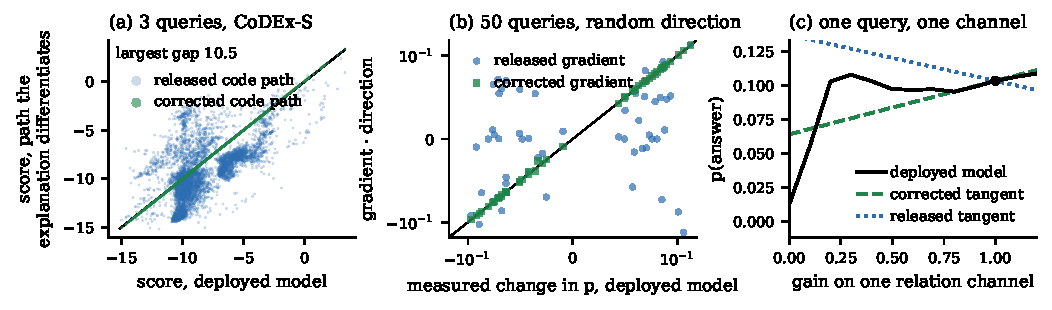
\includegraphics[width=\textwidth]{figs/direction.pdf}
\caption{The released explanation code differentiates a model with its
messages reversed. (a) Every entity's score from the code path the
explanation differentiates, against the deployed model's score: as released
(blue) and on the reversed graph (green). (b) Along one random direction in
edge-weight space per query, the deployed model's measured change in \(p\),
by a central difference, against each gradient's prediction; the line is
exact agreement. (c) One query and one relation channel: \(p\) as the
channel's gain runs from 0 to 1.2, with each gradient's tangent at gain 1.}
\label{fig:direction}
\end{figure*}

ULTRA, like NBFNet's PyTorch Geometric release, runs its layers with a fused
sparse kernel, \texttt{rspmm}, whenever it can. When the edge weights need a
gradient, which is exactly when \texttt{visualize} runs, each layer falls back
to PyTorch Geometric's generic message passing. The two disagree on
direction. The fused kernel sends the message on column \(e\) from
\texttt{edge\_index[1,e]} to \texttt{edge\_index[0,e]}, and the generic path
sends it from \texttt{edge\_index[0,e]} to \texttt{edge\_index[1,e]}. Training
and inference use the kernel, so that is the deployed model. The explanation
differentiates the other one: the same weights with every message running
backwards.

I found this because integrated gradients did not add up. Its attributions
must sum to the change in \(p\) between the empty graph and the full one.
With the released gradient they missed it by a median of
\cxIgRelGapReleased\% of that change on the first \cxIgRelGapN{} CoDEx-S
queries, against \cxIgRelGapCorrected\% with the corrected one. Three checks on \allDirN{}
benchmark queries from CoDEx-S and NELL23k then settle it
(Figure~\ref{fig:direction}). First, the function the explanation
differentiates scores entities up to \allDirGapMax{} logits away from the
deployed model; run on the graph with every edge reversed, the same code
reproduces the deployed scores to within \allDirGapCorrected. Second, along a
random direction in edge-weight space, the corrected gradient predicts the
deployed model's change in \(p\) to a median of \allDirErrCorrected\%, and the
released one misses by a median of \allDirErrReleased\% and has the wrong sign
on \allDirSignReleased{} of the \allDirN{} directions. The corrected error is
not zero because a finite difference in single precision is itself
approximate: with a step of \(10^{-3}\) instead of \(10^{-4}\) it is
\allDirErrCorrectedWide\%. Third, for each query I take the explained
relation channel on which the two gradients disagree most and measure the
slope of \(p\) against that channel's gain at 1. The released gradient has
the wrong sign on \allDirChanSlopeWrongReleased{} of these \allDirChanN{}
channels and the corrected one on \allDirChanSlopeWrongCorrected.

The fix is to run \texttt{visualize} on the reversed graph and map each hop
back to its original edge column. I keep both versions. The released one is
what anyone calling the function gets, so the audit below reports it as
shipped, and the path benchmark is repeated with the corrected one
(Figure~\ref{fig:robust}). The channel gradients and integrated gradients use
the corrected path only.

\section{The benchmark}
\label{sec:bench}

\begin{table*}[t]
\centering\small
\caption{The four graphs. MRR and Hits@\(k\) are filtered, both directions
scored, with ULTRA's own evaluation code, on the number of test triples shown.
``Paper'' is the MRR Galkin et al.\ report for ULTRA pre-trained on three graphs
\cite{ultra}. The \texttt{ultra\_4g} checkpoint used throughout adds NELL-995
to that mixture, so close agreement rather than identity is expected; the
``3g'' column is that paper's own checkpoint, run here on the full test set.
Explained queries are the test triples the frozen model ranks in its top ten,
taken in a fixed random order set before any measurement.}
\label{tab:bench}
\setlength{\tabcolsep}{4.6pt}
\begin{tabular}{lrrrlrcccc rr}
\toprule
graph & entities & relations & edges & \texttt{ultra\_4g} saw it & test scored & MRR & H@10 & paper & 3g & queries & scanned \\
\midrule
WN18RR    & \wnNodes & \wnRelCount & \wnEdges & yes      & \wnBaseN & \wnMrr & \wnHitsTen & 0.480 & n/a & \wnQueries & \wnScanned \\
FB15k-237 & \fbNodes & \fbRelCount & \fbEdges & yes      & \fbBaseN & \fbMrr & \fbHitsTen & 0.368 & n/a & \fbQueries & \fbScanned \\
CoDEx-S   & \cxNodes & \cxRelCount & \cxEdges & held out & \cxBaseN & \cxMrr & \cxHitsTen & 0.472 & \cxTgMrr & \cxQueries & \cxScanned \\
NELL23k   & \nlNodes & \nlRelCount & \nlEdges & held out & \nlBaseN & \nlMrr & \nlHitsTen & 0.239 & \nlTgMrr & \nlQueries & \nlScanned \\
\bottomrule
\end{tabular}
\end{table*}

\textbf{Model and graphs.} ULTRA's \texttt{ultra\_4g} checkpoint, 168{,}705
parameters, frozen, on two CPU cores. It was pre-trained on FB15k-237, WN18RR,
CoDEx-M and NELL-995. WN18RR and FB15k-237 \cite{conve} are therefore in its
mixture; CoDEx-S and NELL23k are not, although each comes from the same source
as a graph that was. Table~\ref{tab:bench} gives the graphs and the
reproduction, which matters first: if the checkpoint did not reproduce, the
thing being explained would not be the published model.

\textbf{Queries.} The test triples are not in the message-passing graph, so an
explanation cannot point at the answer itself. They are taken in a fixed
random order and kept when the model ranks the gold tail in its top ten,
because asking what a prediction rests on only makes sense when the
prediction is right. For each query the beam returns up to 20 candidate
paths; all are deleted individually, and the top 5 form the shortlist.

\textbf{How many queries is enough?} The model is deterministic, so the only
source of variation is which queries are drawn, and every interval below is a
95\% bootstrap over queries. To size the sample I computed each headline
estimate on the first \(n\) queries for growing \(n\), which is a valid sample
because the order was fixed in advance (Figure~\ref{fig:conv}). The estimates
settle and the bands narrow roughly as \(1/\sqrt{n}\). The same analysis shows
what a small study would have risked. On WN18RR the disjoint blocks of five
queries give a ``top path beats chance'' score anywhere from
\wnRelTopGapFiveLo{} to \wnRelTopGapFiveHi{}, and \wnRelTopGapSignNote; at
full size it is \wnRelTopGapEstimate{}, pinned to within
\(\pm\)\wnRelTopGapHalf. Across random splits of the WN18RR queries into two
halves, the two halves' estimates of the shortlist deletion effect differ by
at most \wnRelCompSplitGap{} in 95\% of splits.

\begin{figure*}[t]
\centering
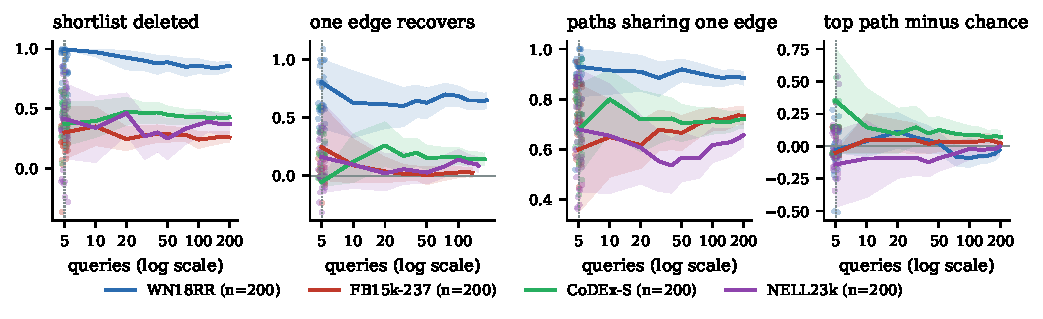
\includegraphics[width=0.94\textwidth]{figs/convergence.pdf}
\caption{Each headline estimate against the number of queries, as one
unbroken line with its 95\% bootstrap band, from \(n = 5\) to the full sample.
The dots at \(n = 5\) are every disjoint block of five queries, which is what a
five-query benchmark could have reported.}
\label{fig:conv}
\end{figure*}

\section{Results}

\begin{table*}[t]
\centering\small
\caption{Main results. Shares are of each query's own starting probability.
Every row uses all 200 queries per graph except the corrected row on FB15k-237
(\fbFxN), integrated gradients (queries where \(\tau\) is defined,
\cxIgN{} and \nlIgN) and the channel rows (\wnNmN, \fbNmN, \cxNmN{} and
\nlNmN).
Brackets are 95\% bootstrap intervals over queries. ``Chance'' is the rate at
which a random path from the pool would be the most damaging one, counting
ties as hits.}
\label{tab:main}
\begin{tabular}{l cccc}
\toprule
 & WN18RR & FB15k-237 & CoDEx-S & NELL23k \\
\midrule
\multicolumn{5}{l}{\emph{set level: are the selected edges load-bearing?}} \\
delete shortlist, share of \(p\) removed & \wnCompFracOfBase{} \ci{\wnCompFracOfBaseCI} & \fbCompFracOfBase{} \ci{\fbCompFracOfBaseCI} & \cxCompFracOfBase{} \ci{\cxCompFracOfBaseCI} & \nlCompFracOfBase{} \ci{\nlCompFracOfBaseCI} \\
delete as many random edges              & \wnCompRandomFracOfBase & \fbCompRandomFracOfBase & \cxCompRandomFracOfBase & \nlCompRandomFracOfBase \\
\midrule
\multicolumn{5}{l}{\emph{ranking: does the order mean anything?}} \\
Kendall \(\tau\), rank against effect    & \wnKendallTauGradVsDrop{} \ci{\wnKendallTauGradVsDropCI} & \fbKendallTauGradVsDrop{} \ci{\fbKendallTauGradVsDropCI} & \cxKendallTauGradVsDrop{} \ci{\cxKendallTauGradVsDropCI} & \nlKendallTauGradVsDrop{} \ci{\nlKendallTauGradVsDropCI} \\
\quad corrected explanation              & \wnFxKendallTauGradVsDrop{} \ci{\wnFxKendallTauGradVsDropCI} & \fbFxKendallTauGradVsDrop{} \ci{\fbFxKendallTauGradVsDropCI} & \cxFxKendallTauGradVsDrop{} \ci{\cxFxKendallTauGradVsDropCI} & \nlFxKendallTauGradVsDrop{} \ci{\nlFxKendallTauGradVsDropCI} \\
\quad integrated gradients               & n/a & n/a & \cxIgTau{} \ci{\cxIgTauCI} & \nlIgTau{} \ci{\nlIgTauCI} \\
top path is the most damaging            & \wnTopOneIsBest & \fbTopOneIsBest & \cxTopOneIsBest & \nlTopOneIsBest \\
\quad chance                             & \wnTopOneChance & \fbTopOneChance & \cxTopOneChance & \nlTopOneChance \\
\midrule
\multicolumn{5}{l}{\emph{relation channels, corrected gradient}} \\
silence strongest explained channel      & \wnNmBest & \fbNmBest & \cxNmBest & \nlNmBest \\
silence a random channel                 & \wnNmRandom & \fbNmRandom & \cxNmRandom & \nlNmRandom \\
share of effect present at half gain     & \wnNmHalfDose & \fbNmHalfDose & \cxNmHalfDose & \nlNmHalfDose \\
gradient has the sign of silencing       & \wnNmSignAgree\% & \fbNmSignAgree\% & \cxNmSignAgree\% & \nlNmSignAgree\% \\
strongest channel is the query relation  & \wnNmTopQueryRel\% & \fbNmTopQueryRel\% & \cxNmTopQueryRel\% & \nlNmTopQueryRel\% \\
\midrule
\multicolumn{5}{l}{\emph{redundancy: many explanations or one?}} \\
paths sharing the busiest edge           & \wnBottleneckFrac & \fbBottleneckFrac & \cxBottleneckFrac & \nlBottleneckFrac \\
distinct edges / edges listed            & \wnDistinctEdgeRatio & \fbDistinctEdgeRatio & \cxDistinctEdgeRatio & \nlDistinctEdgeRatio \\
that one edge recovers                   & \wnSingleEdgeRecoversFrac{} \ci{\wnSingleEdgeRecoversFracCI} & \fbSingleEdgeRecoversFrac{} \ci{\fbSingleEdgeRecoversFracCI} & \cxSingleEdgeRecoversFrac{} \ci{\cxSingleEdgeRecoversFracCI} & \nlSingleEdgeRecoversFrac{} \ci{\nlSingleEdgeRecoversFracCI} \\
\midrule
\multicolumn{5}{l}{\emph{structure of the queries}} \\
reverse fact already in graph            & \wnRevPct\% & \fbRevPct\% & \cxRevPct\% & \nlRevPct\% \\
median tail degree                       & \wnTailDegMedian & \fbTailDegMedian & \cxTailDegMedian & \nlTailDegMedian \\
\bottomrule
\end{tabular}
\end{table*}

\subsection{The selected edges are load-bearing}

The result that goes the method's way comes first, and it holds everywhere.
Deleting the shortlist removes \wnCompFracOfBase{} of the gold tail's
probability on WN18RR, \fbCompFracOfBase{} on FB15k-237, \cxCompFracOfBase{} on
CoDEx-S and \nlCompFracOfBase{} on NELL23k (Table~\ref{tab:main}). Deleting the
same number of random edges removes nothing measurable on any graph. The
gradient is pointing at part of the graph the model depends on, and that is
not a given.

Keeping only the shortlist does not give a clean answer in the other
direction. With a handful of edges left, most rival entities are cut off too,
so the gold tail can gain probability just because it has fewer competitors.
It does on \wnFracSuffAboveOne\% of WN18RR queries, \fbFracSuffAboveOne\% of
FB15k-237, \cxFracSuffAboveOne\% of CoDEx-S and \nlFracSuffAboveOne\% of
NELL23k. I report the retained share for completeness and draw no conclusion
about sufficiency from it. For a model that takes a softmax over every entity,
a deletion test of necessity is well posed and a keep-only test is not.

\begin{figure*}[t]
\centering
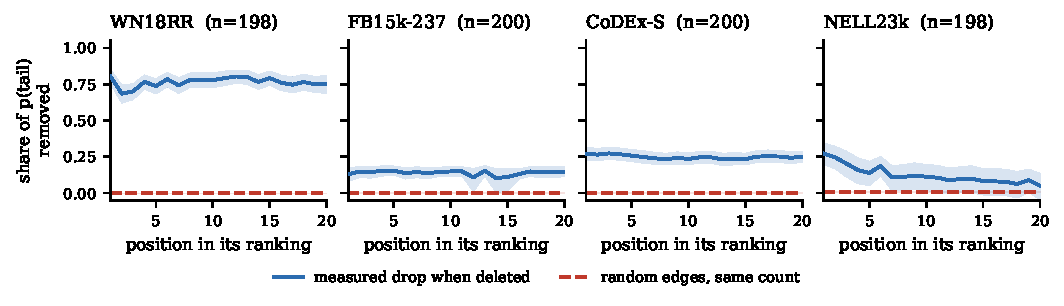
\includegraphics[width=\textwidth]{figs/rank_vs_drop.pdf}
\caption{What the method ranks first is not what matters most. The horizontal
axis walks down the method's own ordering of its 20 candidates; the vertical
axis is the share of the gold tail's probability that deleting that path
removes, with a 95\% bootstrap band. A faithful ranking would fall from left to
right. The dashed line deletes the same number of random edges.}
\label{fig:rankdrop}
\end{figure*}

\subsection{As released, the order is close to meaningless}

A faithful ranking would make Kendall's \(\tau\) between the method's order and
the measured drop close to 1. It is \wnKendallTauGradVsDrop{} on WN18RR,
\fbKendallTauGradVsDrop{} on FB15k-237, \cxKendallTauGradVsDrop{} on CoDEx-S
and \nlKendallTauGradVsDrop{} on NELL23k. Figure~\ref{fig:rankdrop} shows it
directly: walking down the method's own list, the effect of deleting each path
stays flat. The plainest version of the question is how often the path ranked
first is actually the most damaging one to delete. On WN18RR it is
\wnTopOneIsBest{} against a chance rate of \wnTopOneChance{}, no better than
a random pick; on the other graphs it is at or modestly above chance. This is the shape of Hase et al.'s result one domain
over \cite{hase}: a quantity read from the model's internals that correlates
with what the model does is not thereby a measurement of what it depends on.

\begin{figure*}[t]
\centering
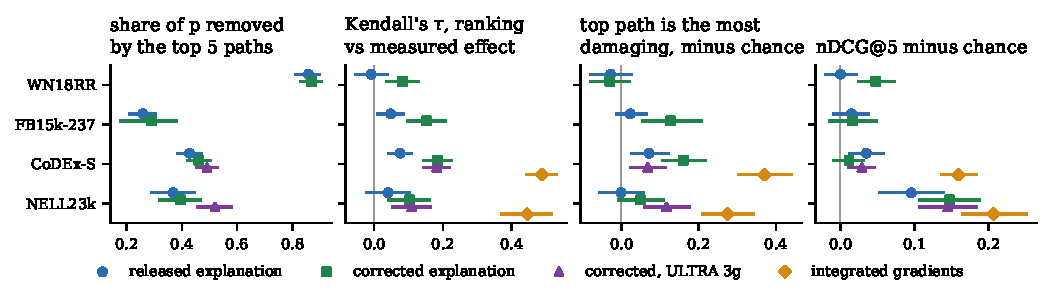
\includegraphics[width=\textwidth]{figs/robustness.pdf}
\caption{The headline numbers, one variable changed at a time: the released
explanation, the direction-corrected one, the corrected one on ULTRA's
three-graph checkpoint, and integrated gradients re-ranking the corrected
explanation's own candidates. Points are means over queries, lines 95\%
bootstrap intervals. Integrated gradients was run on the held-out graphs only,
and it re-ranks a fixed candidate set, so it has no joint-deletion value.}
\label{fig:robust}
\end{figure*}

\subsection{Fixing the direction helps the order, a little}

Repeating the benchmark with the corrected explanation leaves the set-level
result where it was (Figure~\ref{fig:robust}): its shortlist removes
\cxFxCompFracOfBase{} of the gold tail's probability on CoDEx-S and
\nlFxCompFracOfBase{} on NELL23k, against \cxCompFracOfBase{} and
\nlCompFracOfBase{} as released. The order improves. On the same queries
Kendall's \(\tau\) rises from \cxFxPairedRel{} to \cxFxPairedFix{} on CoDEx-S,
a gain of \cxFxTauGain{} \ci{\cxFxTauGainCI}, and from \nlFxPairedRel{} to
\nlFxPairedFix{} on NELL23k, a gain of \nlFxTauGain{} \ci{\nlFxTauGainCI}; on
the seen graphs the gain is \wnFxTauGain{} and \fbFxTauGain. So the bug explains part of why the order was
poor, but not most of it: the right gradient of the right model still ranks
paths far from their measured effect. ULTRA's three-graph checkpoint, the
model of the ULTRA paper, gives the same picture, with \(\tau\) of
\cxTgKendallTauGradVsDrop{} and \nlTgKendallTauGradVsDrop, and it reproduces
that paper's MRR, \cxTgMrr{} against 0.472 on CoDEx-S and \nlTgMrr{} against
0.239 on NELL23k (Table~\ref{tab:bench}).

\subsection{Integrated gradients rank better, but not well}

The gradient is a slope at the point where every edge weight is one.
Integrated gradients average that slope along the way from the empty graph to
the full one \cite{ig}. Re-ranking the corrected explanation's own candidates
by the integrated gradients summed over each path's edges raises \(\tau\) from
\cxIgGradTau{} to \cxIgTau{} on CoDEx-S, a paired gain of \cxIgTauGain{}
\ci{\cxIgTauGainCI}, and from \nlIgGradTau{} to \nlIgTau{} on the \nlIgN{}
NELL23k queries where both are defined. How often the top path is the most
damaging one, above chance, goes from \cxIgGradTopGap{} to \cxIgTopGap{} on
CoDEx-S. Summed over a relation channel's edges, integrated gradients have
the sign of that channel's silencing effect on \cxIgChanSign\% of the
channels that matter, against \cxIgChanGradSign\% for the gradient, both
averaged per query as in Table~\ref{tab:main}. It costs 16 backward passes
instead of one, and with 16 steps the attributions add up to the total change
only to within a median of \cxIgCompGapRel\% of it, so the integral is
approximate. This is the largest improvement in the study, and it still leaves
\(\tau\) near 0.5 at best: the order of the paths is only loosely tied to what
deleting them does.

\begin{figure*}[t]
\centering
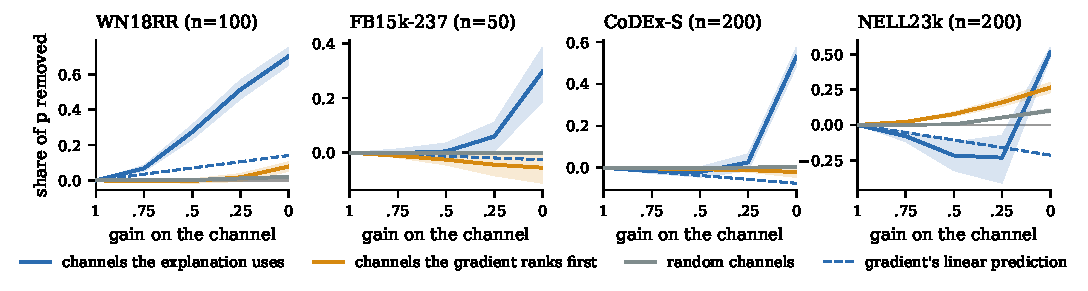
\includegraphics[width=\textwidth]{figs/dose_response.pdf}
\caption{Turning one relation channel down from gain 1 to 0. Curves are the
share of the gold tail's probability removed, averaged over queries, with 95\%
bootstrap bands, for the channels the explanation's paths use, the other
channels the corrected gradient ranks highest, and random channels. The dashed
line is the gradient's linear prediction for the explained channels.}
\label{fig:dose}
\end{figure*}

\subsection{Relation channels are switches, not dials}

Turning a channel down shows why a slope misleads (Figure~\ref{fig:dose}).
Silencing the strongest channel the explanation uses removes \cxNmBest{} of
the gold tail's probability on CoDEx-S and \nlNmBest{} on NELL23k, while a
random channel removes \cxNmRandom{} and \nlNmRandom{} (Table~\ref{tab:main}).
The response is not a dial. For channels whose silencing matters, only
\cxNmHalfDose{} of the full effect is present at half gain on CoDEx-S, where a
straight line would give 0.5. \cxNmSwitch\% of them have less than a quarter
of it, and \cxNmInvertedU\% change direction somewhere along the dose, a
non-monotone response like dopamine's inverted U \cite{cools2011}. Turning
every explained channel down to half together removes nothing measurable on
CoDEx-S (\cxNmJointHalf{} \ci{\cxNmJointHalfCI}) and raises \(p\) on NELL23k
(\nlNmJointHalf), against \cxNmJoint{} at zero on CoDEx-S. WN18RR is the
exception: there half gain on the explained channels already removes
\wnNmJointHalf, about what a straight line gives. A slope taken at gain 1
cannot see a switch that sits near 0, and the corrected gradient has the sign
of the silencing effect for only \cxNmSignAgree\% of these channels on
CoDEx-S and \nlNmSignAgree\% on NELL23k, where chance is about half. The
channel that matters most is usually the query's own relation, from
\nlNmTopQueryRel\% of queries on NELL23k to \cxNmTopQueryRel\% on CoDEx-S.
The paths do name that relation, as a hop; what they cannot show is that it
acts as a switch. This is
the Topic~8 result again, one level up: the gradient localises a channel, and
localising it does not predict what editing it does.

\subsection{One edge or many depends on the graph}

The shortlist is presented as several independent paths. On WN18RR it is close
to one. A single edge runs through \wnBottleneckFrac{} of the listed paths, only
\wnDistinctEdgeRatio{} of the listed edge slots are distinct, and deleting that
one edge reproduces \wnSingleEdgeRecoversFrac{} of the effect of deleting the
whole shortlist. The obvious objection is that these tails are poorly
connected so that any deletion strands them; it fails, since the median tail
degree is \wnTailDegMedian{} and the result holds on tails of degree four or
more (\wnSingleEdgeRecoversHiDeg).

The other graphs do not look like this. On FB15k-237 the busiest edge appears
in \fbBottleneckFrac{} of paths and deleting it recovers
\fbSingleEdgeRecoversFrac{} of the effect, an interval that includes zero; the
paths there are genuinely different routes. The structural difference is
in the graphs themselves (Tables~\ref{tab:bench} and~\ref{tab:main}): WN18RR is sparse, has \wnRelCount{} relation
types and keeps symmetric relations, so \wnRevPct\% of its queries have their
reverse fact in the graph, while FB15k-237 has \fbRelCount{} relation types, a
median tail degree of \fbTailDegMedian{}, and \fbRevPct\% of queries with a
reverse fact. The held-out graphs sit between the two and let the pattern be
checked on graphs the model never saw.

\begin{table}[t]
\centering\small
\caption{WN18RR split on whether the query's reverse fact is in the training
graph. The forward edge is never present (\wnFwdPct\%).}
\label{tab:sym}
\begin{tabular}{lcc}
\toprule
 & reverse present & reverse absent \\
 & (\wnRevN{} queries) & (\wnNoRevN{} queries) \\
\midrule
paths sharing one edge & \wnRevBottleneckFrac & \wnNoRevBottleneckFrac \\
Kendall \(\tau\)       & \wnRevKendallTauGradVsDrop & \wnNoRevKendallTauGradVsDrop \\
top path is best       & \wnRevTopOneIsBest & \wnNoRevTopOneIsBest \\
\quad chance           & \wnRevTopOneChance & \wnNoRevTopOneChance \\
one edge recovers      & \wnRevSingleEdgeRecoversFrac & \wnNoRevSingleEdgeRecoversFrac \\
rewire, old loses      & \wnRevRewireDropOnGold & \wnNoRevRewireDropOnGold \\
\bottomrule
\end{tabular}
\end{table}

\subsection{The control I found by reading an example}
\label{sec:sym}

% generated by pathfaith.case_study
\begin{table*}[t]
\centering\small
\caption{A worked example, the first query in the benchmark's fixed order that meets the rule in its heading, re-run under the benchmark protocol. Arrows show the direction of the stored fact, so a leftward arrow is a hop taken backwards along a reverse edge. Names are from the WN18RR text release.}
\label{tab:case}
\begin{tabular}{@{}p{0.2\textwidth}p{0.76\textwidth}@{}}
\toprule
\multicolumn{2}{@{}p{0.97\textwidth}@{}}{\textbf{WN18RR, first query with its reverse fact in the graph}.\quad Query: sociology \(-\)\,derivationally related form\,\(\rightarrow\) ?\quad answer \textbf{sociologist}, rank 1, \(p = 0.196\)} \\
path 1 (1 hop) & sociology \(\leftarrow\)\,{\scriptsize derivationally related form}\,\(-\) sociologist \\
path 2 (3 hops) & sociology \(\leftarrow\)\,{\scriptsize synset domain topic of}\,\(-\) mores \\ & mores \(-\)\,{\scriptsize synset domain topic of}\,\(\rightarrow\) sociology \\ & sociology \(\leftarrow\)\,{\scriptsize derivationally related form}\,\(-\) sociologist \\
path 3 (5 hops) & sociology \(\leftarrow\)\,{\scriptsize synset domain topic of}\,\(-\) mores \\ & mores \(-\)\,{\scriptsize synset domain topic of}\,\(\rightarrow\) sociology \\ & sociology \(\leftarrow\)\,{\scriptsize synset domain topic of}\,\(-\) mores \\ & mores \(-\)\,{\scriptsize synset domain topic of}\,\(\rightarrow\) sociology \\ & sociology \(\leftarrow\)\,{\scriptsize derivationally related form}\,\(-\) sociologist \\
\addlinespace[2pt]
delete top 5 (6 edges) & \(p\) 0.196 \(\rightarrow\) 0.000, rank 1 \(\rightarrow\) 24859 \\
delete busiest edge only & \(p\) 0.196 \(\rightarrow\) 0.000, rank 1 \(\rightarrow\) 24874: 100\% of that effect \\
 & {\footnotesize that edge, in 4 of 5 paths: sociologist \(-\)\,{\scriptsize derivationally related form}\,\(\rightarrow\) sociology} \\
\bottomrule
\end{tabular}
\end{table*}


While building a worked example on WN18RR, the top ``path'' came back as a
single hop, and that hop was the stored reverse of a training fact.
Table~\ref{tab:case} shows the first such query in the benchmark's order. The
model is asked what \emph{sociology} is derivationally related to and answers
\emph{sociologist}, because the training graph already holds that fact the
other way round. The explanation offers five paths. Two of them detour from
sociology to \emph{mores} and straight back before taking the same reverse
hop, and deleting that one hop alone does everything that deleting all five
paths does. This is not leakage, since the test edge itself is never in the
graph, but it changes what there is to explain, so Table~\ref{tab:sym} splits
WN18RR on it. Two findings survive the split: the
paths funnel through one edge on both halves, and the ranking is no better
than chance on both. What does not survive is how much that edge carries,
\wnRevSingleEdgeRecoversFrac{} with the reverse fact present against
\wnNoRevSingleEdgeRecoversFrac{} without, and almost all of the rewire effect.
The first column is the sharpest thing in this paper. On those queries the
model is doing a one-hop lookup, and the interface returns up to 20 paths of
up to six hops. Nothing in that output says the answer came from one
reverse lookup, which is the one thing a reader would most want to know.

\subsection{Rerouting a path destroys rather than redirects}

If the top path were the mechanism, pointing its last hop at another entity
should carry the answer there. On WN18RR the old answer loses
\wnRewireDropOnGold{} of probability while the new target gains
\wnRewireGainOnTarget{}, and the effect comes almost entirely from the
reverse-fact queries; elsewhere the rewire barely moves either (the old answer
loses at most \nlRewireDropOnGold{} on NELL23k). Removing the hop takes away support without
transferring it, which is MQuAKE's portability failure \cite{mquake} in a
setting where the edit is exact.

\section{Discussion}

The bug is the most concrete finding, and its lesson is general. A gradient
explanation is a statement about whatever code was differentiated, and here
that was not the code that makes the predictions. Nothing in the output looks
wrong, and the deletion tests did not catch it. Checking the gradient against
the model's own response did: the completeness of integrated gradients, then
the scores and a finite difference.

The gradient finds a region of the graph the model depends on, and random
deletion confirms it is not luck. As released it ranks little or nothing
inside that region, and even fixed it ranks poorly; whether it decomposes the
region into separate evidence depends on the graph. A heat map over edges and a ranked list of reasoning chains are
different promises. NBFNet's gradient keeps the first and is presented as the
second.

The redundancy result is the one I would hand to someone building on this. Ten
paths that agree feel like ten witnesses. If nine are the same witness in
different coats, a reader who spot-checks two and finds them sound has learned
far less than they think, and the output looks the same whether that is
happening or not. Five changes would help: run the explanation on the reversed
graph; rank with integrated gradients, at 16 backward passes, if an order is
going to be shown; report the busiest edge and confirm it with one deletion;
print the distinct-edge count beside any list of paths; and flag queries whose
reverse fact is already in the graph.

None of this says the model is broken. Its accuracy is in line with what the
ULTRA paper reports, and the edges its gradient selects are load-bearing. What
fails is the explanation layer: first a gradient taken through the wrong code
path, and then, once that is fixed, a real but coarse signal over edges,
served as a ranked list of discrete reasoning chains it does not support. The
channel experiment suggests why a better gradient is not enough: much of the
answer rides on relation channels that act as switches, which a slope cannot
see.

\section{Limitations}

\textbf{Overlapping paths.} Deleting a path disturbs other paths that share its
edges, so a single-path drop is not cleanly that path's. The redundancy rows
of Table~\ref{tab:main} measure this, and the set-level and single-edge
numbers do not depend on it. \textbf{One model family}, four graphs:
the claim is about this family's explanations, not path reasoning in general.
\textbf{Correct predictions only}: what the explanation does on the model's
mistakes is a separate question. \textbf{Smaller runs on the seen graphs}: the corrected benchmark has
\fbFxN{} queries on FB15k-237 and the channel experiment \wnNmN{} on WN18RR
and \fbNmN{} on FB15k-237, against 200 elsewhere; integrated gradients and the
second checkpoint were run on the held-out graphs only. \textbf{Integrated
gradients with 16 steps}: completeness holds to a median of
\cxIgCompGapRel\% of the total change on CoDEx-S; more steps would tighten
it. \textbf{NBFNet-PyG}: its layer code has the same fallback, but I ran the
checks on ULTRA only.
\textbf{WN18RR node merges}: the release PyTorch Geometric loads merges 161
unrelated synsets (0.4\%) into shared nodes; the checkpoint was trained on
that graph, so I left it.

\section{Conclusion}

I tested whether the paths NBFNet reports are the paths it relies on, by
editing a frozen checkpoint's graph rather than reading its gradients, on
\allQueries{} queries over four graphs. The released explanation
differentiates the model with its messages reversed; fixed, it matches the
deployed model. Either way the selected edges are load-bearing, and the order
they come in carries little: the fix and integrated gradients each improve
it, and neither makes it faithful. Localising is not explaining, and only
changing the graph tells the two apart.

{\small
\bibliographystyle{ieeenat_fullname}
\bibliography{refs}
}

\end{document}
